\section{Mythes et précurseurs}
Depuis l'Antiquité, l'humanité rêve de voler. Le mythe d'Icare illustre cette fascination pour le vol, mêlée de danger et d'audace. Les inventions comme le cerf-volant chinois (-200 av. J.-C.) et les études visionnaires de Léonard de Vinci (XVe siècle) montrent que ce rêve traverse les civilisations. Au XVIIIe siècle, les travaux scientifiques de George Cayley posent les bases de l'aérodynamique moderne, identifiant les quatre forces du vol. Ces précurseurs ont ouvert la voie aux pionniers qui réaliseront enfin le rêve ancestral de l'humanité.
\begin{table}[H]
    \centering
    \begin{tabular}{c l c}
        \begin{minipage}{.075\textwidth}
            \begin{figure}[H]
            \setlength{\belowcaptionskip}{-40pt}
                \centering
                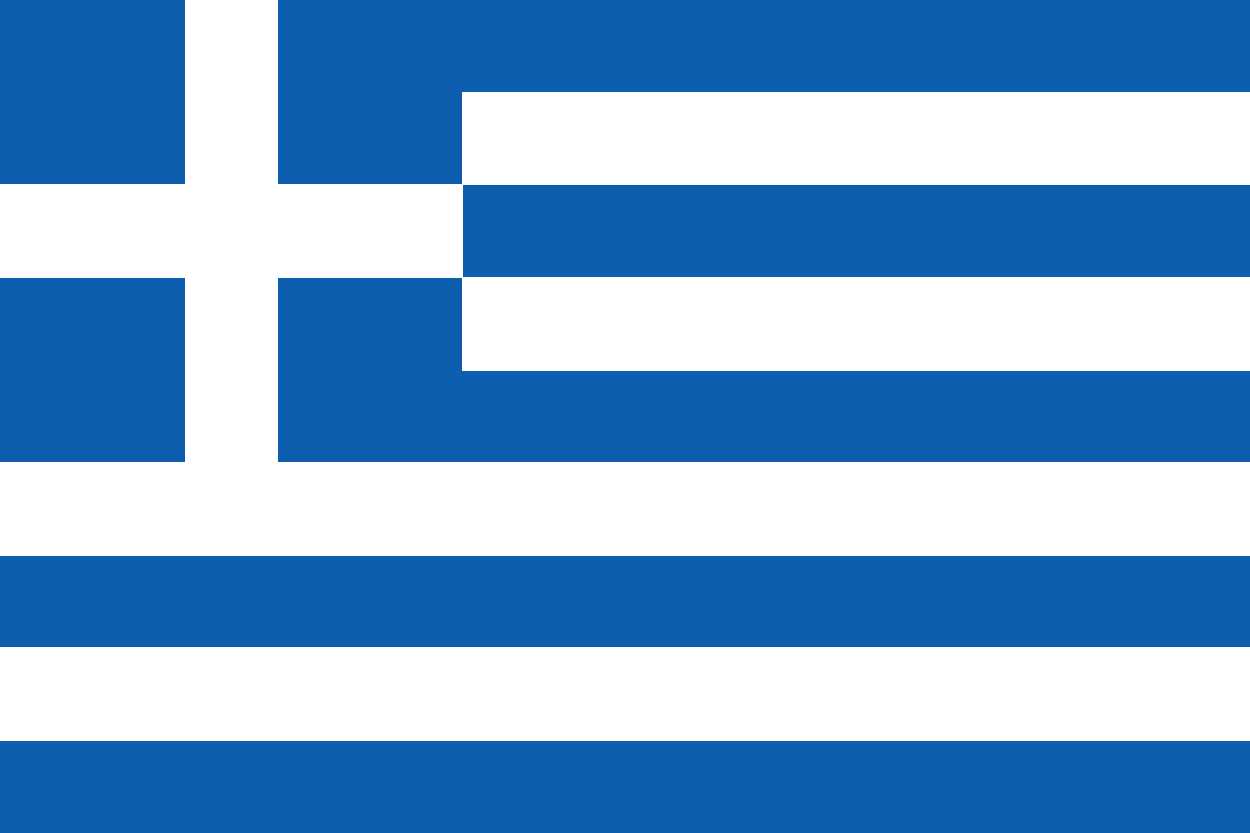
\includegraphics[width=1.0\linewidth]{Annexes/friseChronologique/img/Flag_of_Greece.pdf}
                \captionsetup{labelformat=empty}\refDrapeau{Drapeau Greece}{frise:Flag_of_Greece.pdf}
            \end{figure}
        \end{minipage}
    &
        \begin{minipage}{.65\textwidth}
            \textbf{-800} - \textbf{Le mythe d'Icare}
            
            Dans la mythologie grecque, Dédale fabrique des ailes en plumes et en cire pour lui et son fils Icare afin de s'échapper du labyrinthe. Icare, s'approchant trop près du soleil, voit la cire fondre et tombe dans la mer. Ce mythe illustre depuis l'Antiquité le rêve ancestral de l'Homme de voler.
            \begin{figure}[H]
                \legende{Icare et Dédale}{frise:Anthony_van_Dyck_-_Daedalus_and_Icarus_-_Google_Art_Project.jpg}
            \end{figure}
        \end{minipage}
    &
        \begin{minipage}{.275\textwidth}
            \begin{figure}[H]
                \centering
                \includegraphics[width=1.0\linewidth]{Annexes/friseChronologique/img/Anthony_van_Dyck_-_Daedalus_and_Icarus_-_Google_Art_Project.jpg}
            \end{figure}
        \end{minipage}
    \end{tabular}
\end{table}
\begin{table}[H]
    \centering
    \begin{tabular}{c l c}
        \begin{minipage}{.075\textwidth}
            \begin{figure}[H]
            \setlength{\belowcaptionskip}{-40pt}
                \centering
                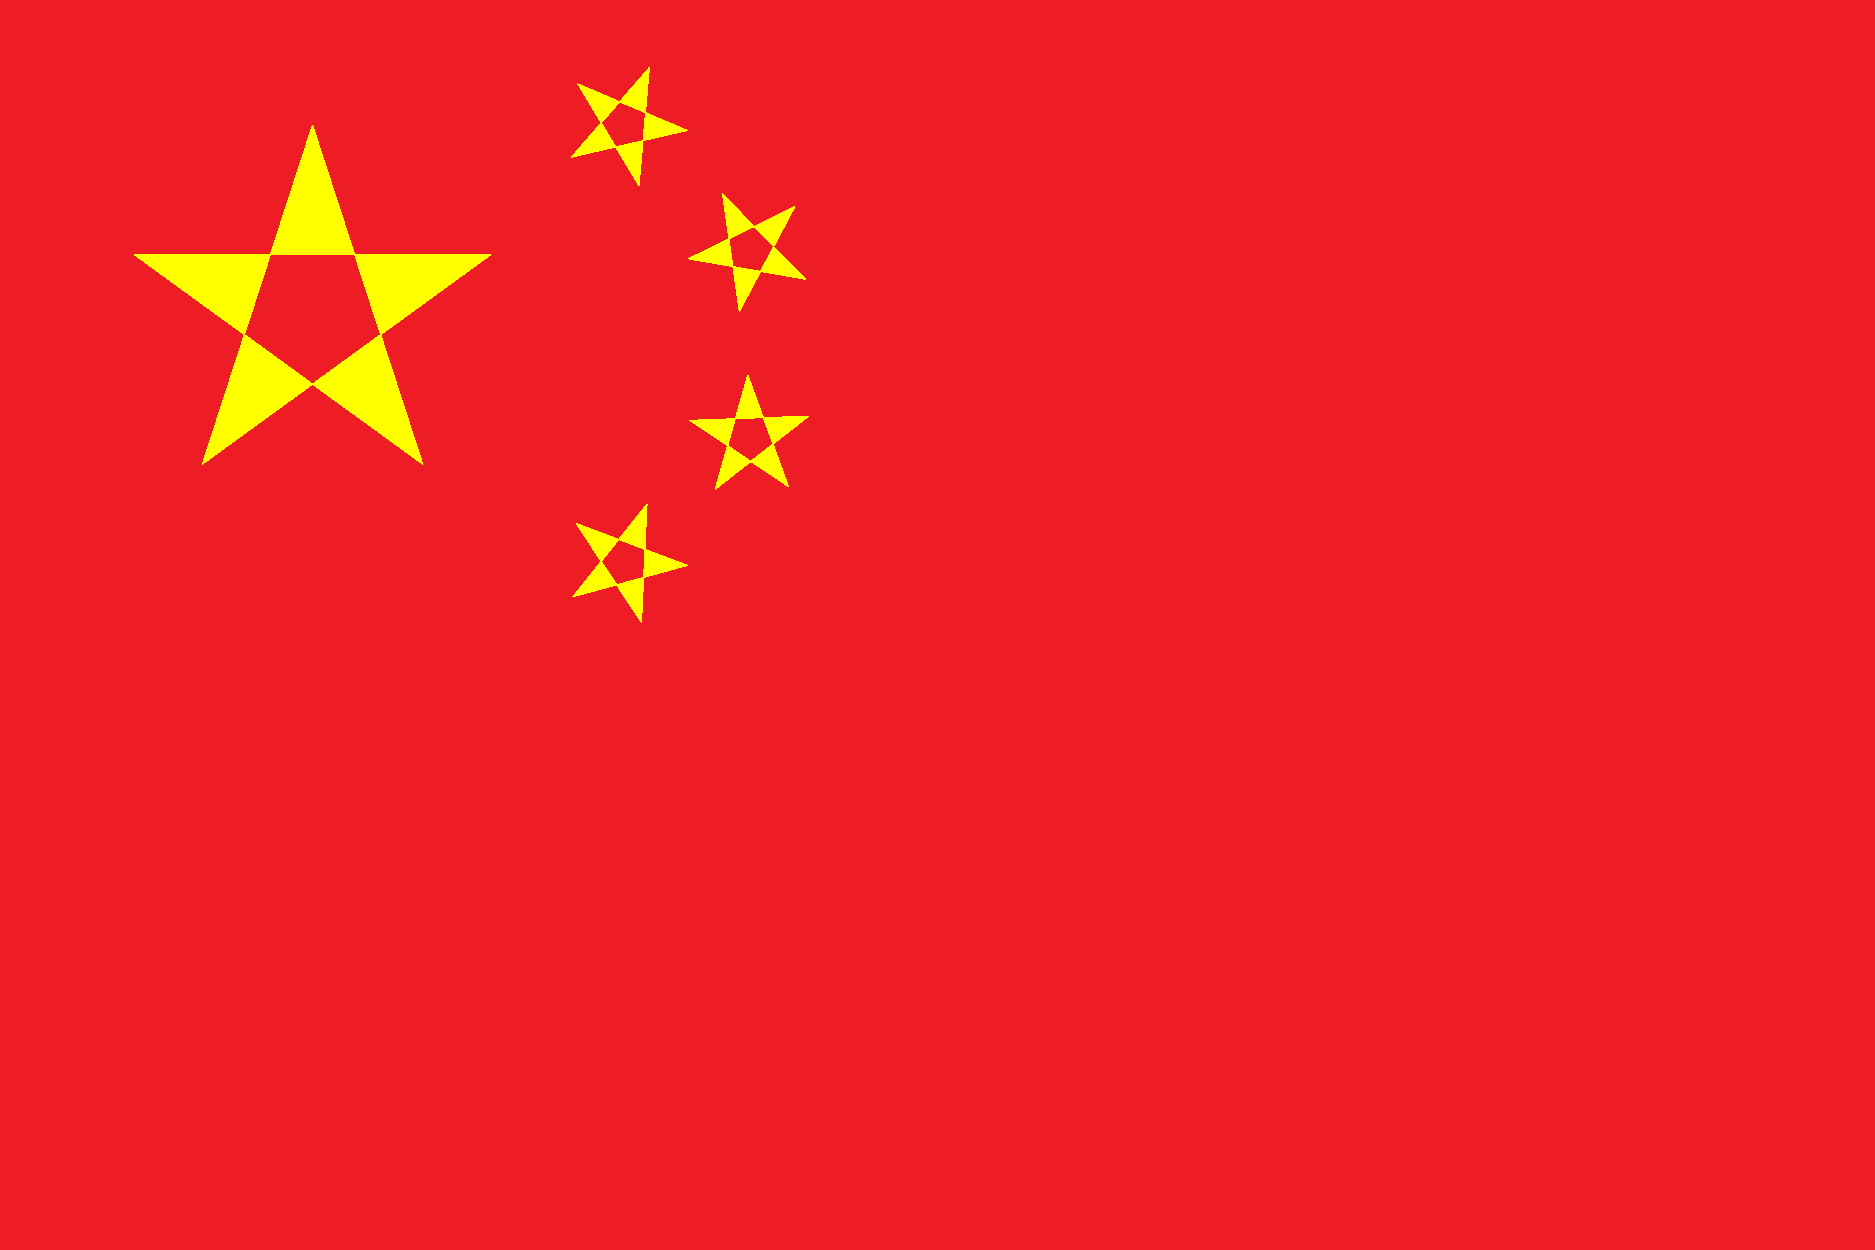
\includegraphics[width=1.0\linewidth]{Annexes/friseChronologique/img/Flag_of_the_People27s_Republic_of_China.pdf}
                \captionsetup{labelformat=empty}\refDrapeau{Drapeau the People27s Republic of China}{frise:Flag_of_the_People27s_Republic_of_China.pdf}
            \end{figure}
        \end{minipage}
    &
        \begin{minipage}{.65\textwidth}
            \textbf{-200} - \textbf{Invention du cerf-volant}
            
            Le cerf-volant est inventé en Chine vers 200 avant J.-C. Il sera utilisé pendant des siècles pour des applications militaires, religieuses et scientifiques. Au XVIIIe siècle, les cerfs-volants serviront aux premières expériences scientifiques sur l'aérodynamique.
            \begin{figure}[H]
                \legende{Cerf-volant moderne}{frise:Chinese_Kite.jpg}
            \end{figure}
        \end{minipage}
    &
        \begin{minipage}{.275\textwidth}
            \begin{figure}[H]
                \centering
                \includegraphics[width=1.0\linewidth]{Annexes/friseChronologique/img/Chinese_Kite.jpg}
            \end{figure}
        \end{minipage}
    \end{tabular}
\end{table}
\begin{table}[H]
    \centering
    \begin{tabular}{c l c}
        \begin{minipage}{.075\textwidth}
            \begin{figure}[H]
            \setlength{\belowcaptionskip}{-40pt}
                \centering
                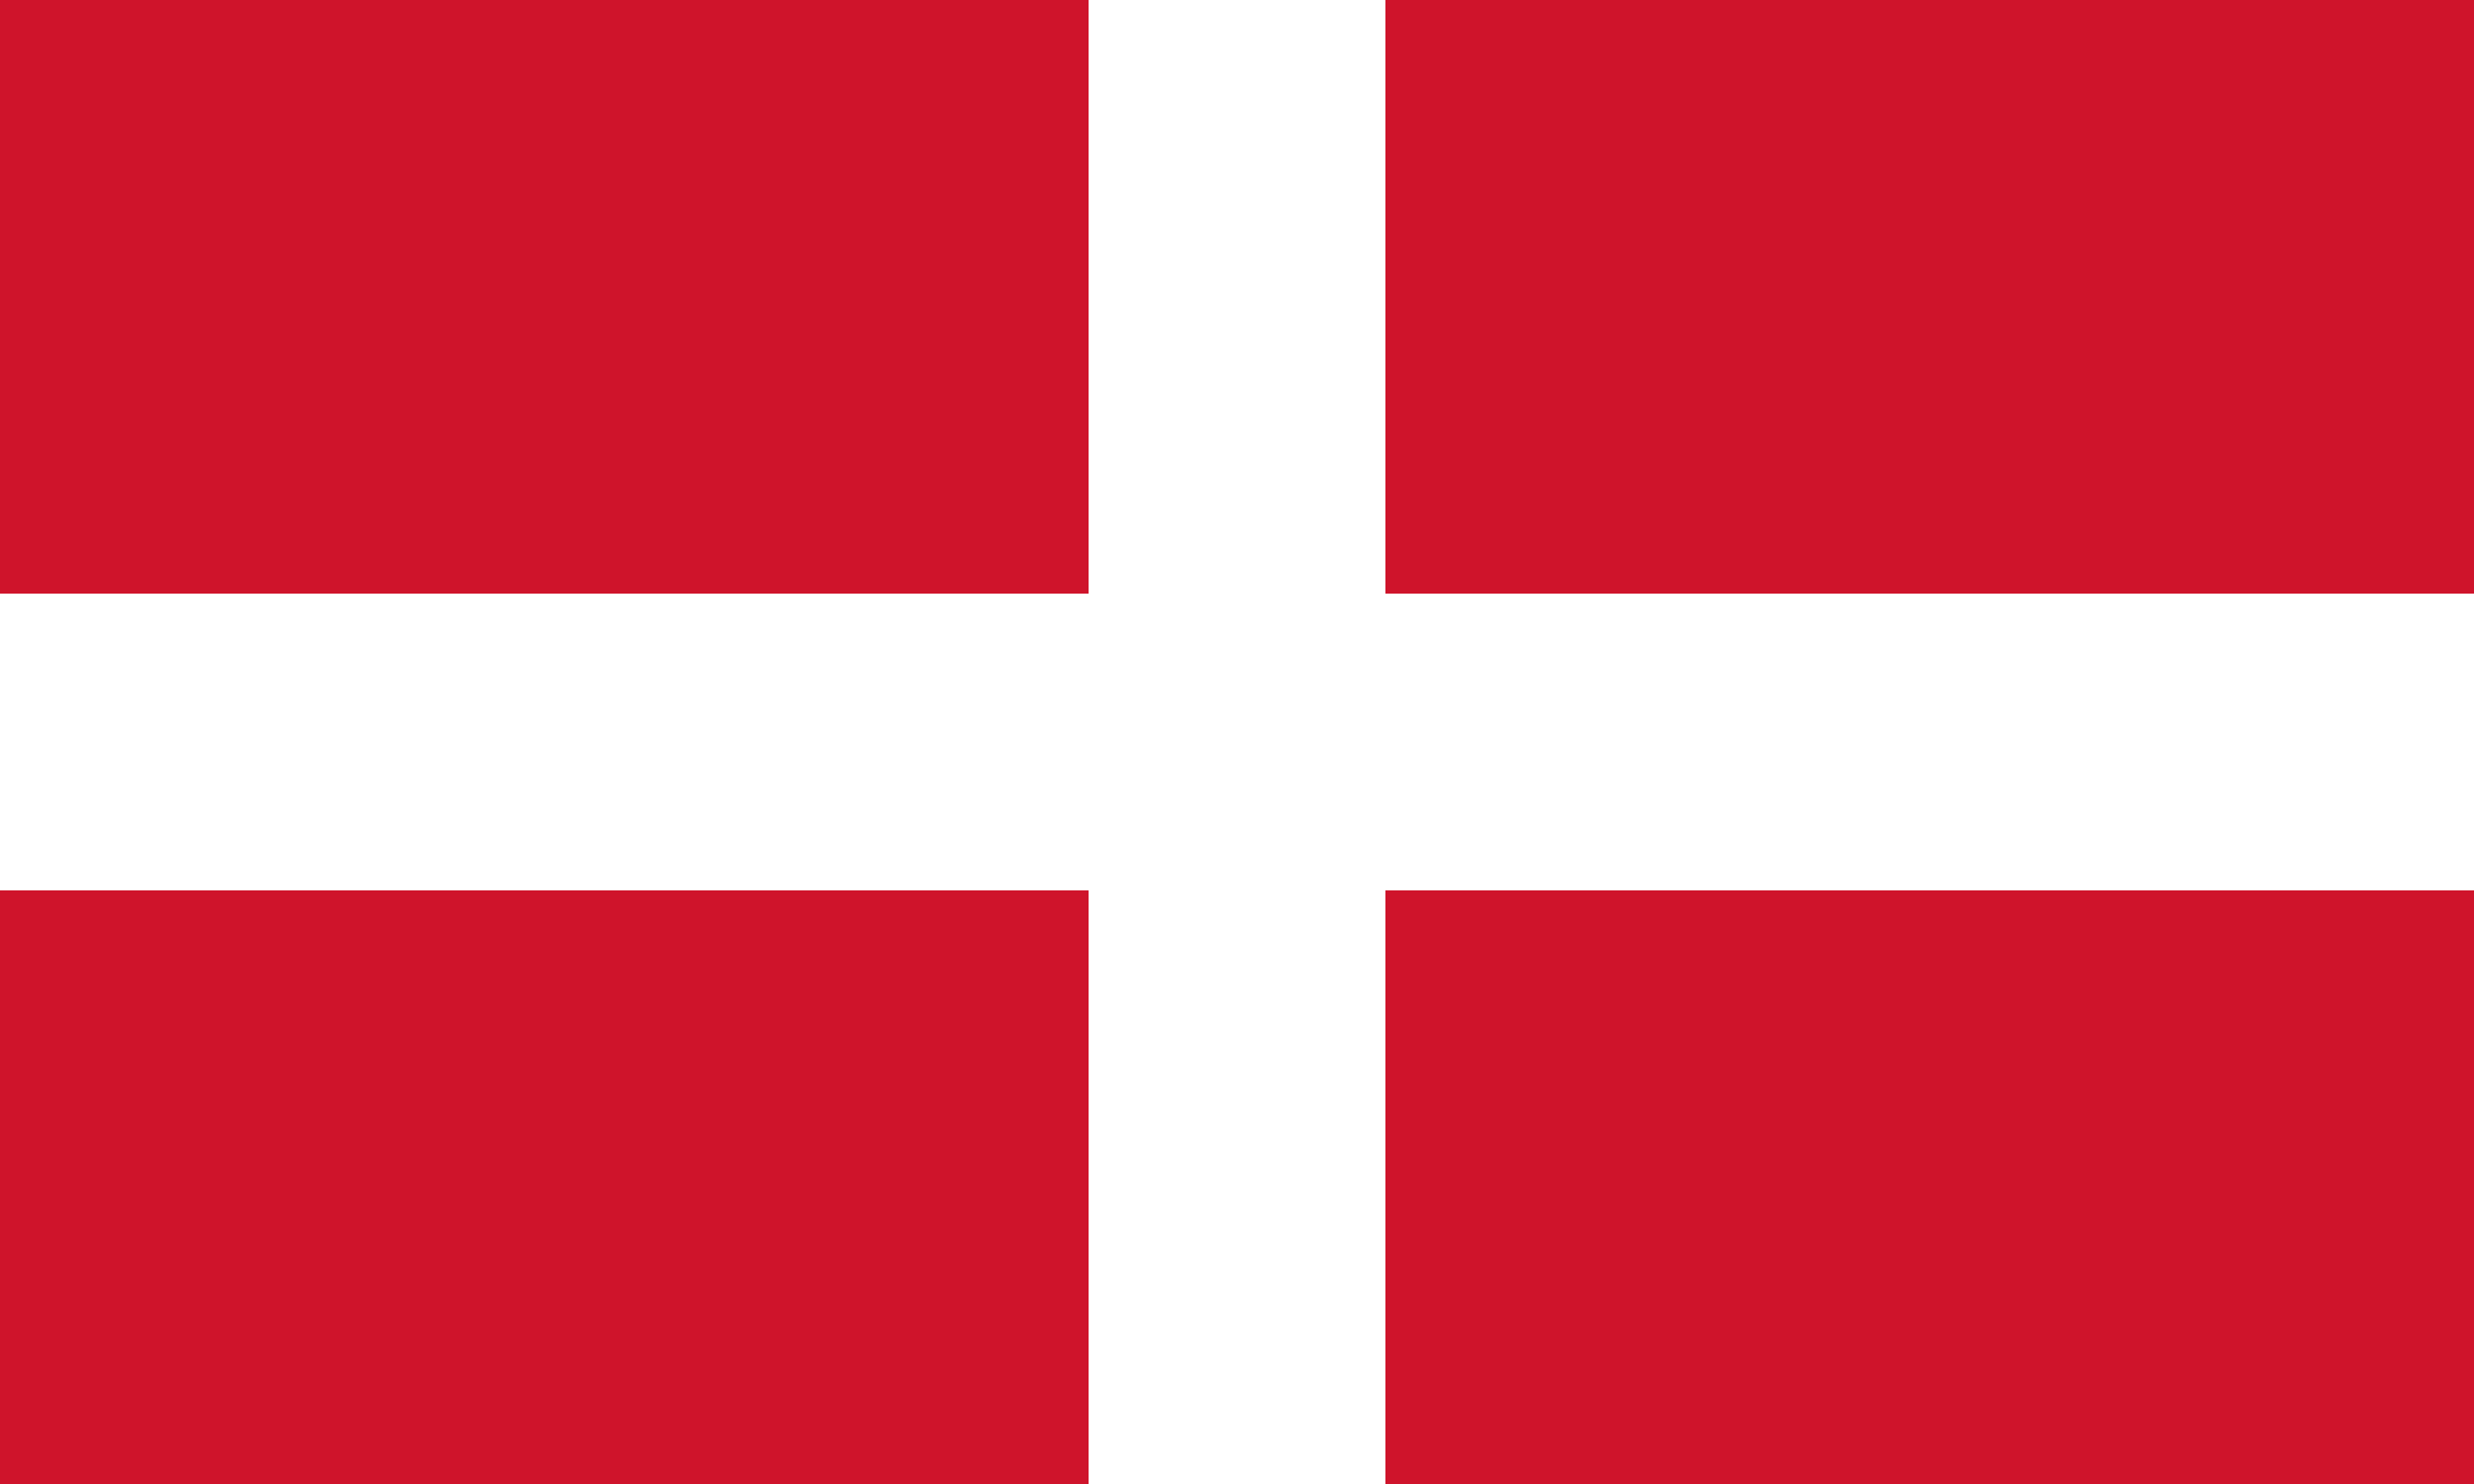
\includegraphics[width=1.0\linewidth]{Annexes/friseChronologique/img/Flag_of_John_the_Baptist.pdf}
                \captionsetup{labelformat=empty}\refDrapeau{Drapeau John the Baptist}{frise:Flag_of_John_the_Baptist.pdf}
            \end{figure}
        \end{minipage}
    &
        \begin{minipage}{.65\textwidth}
            \textbf{1485} - \textbf{Léonard de Vinci, visionnaire du vol}
            
            Léonard de Vinci étudie le vol des oiseaux et conçoit de nombreuses machines volantes dans ses carnets : l'ornithoptère (machine à ailes battantes), le parachute pyramidal, et une vis aérienne (ancêtre de l'hélicoptère). Bien que jamais construites de son vivant, ses études pionnières influenceront les inventeurs futurs.
            \begin{figure}[H]
                \legende{Étude de la vis aérienne de Léonard de Vinci}{frise:Leonardo_helicopter.JPG}
            \end{figure}
        \end{minipage}
    &
        \begin{minipage}{.275\textwidth}
            \begin{figure}[H]
                \centering
                \includegraphics[width=1.0\linewidth]{Annexes/friseChronologique/img/Leonardo_helicopter.JPG}
            \end{figure}
        \end{minipage}
    \end{tabular}
\end{table}
\section{L'aérostation}
L'ère de l'aérostation débute en 1783 avec le vol historique de la montgolfière des frères Montgolfier, suivi rapidement par le ballon à gaz de Jacques Charles. Ces "plus légers que l'air" permettent les premières aventures humaines dans le ciel : traversées, records d'altitude, applications militaires et même les premières photographies aériennes par Nadar en 1858. Les ballons captifs servent à l'observation, tandis que les dirigeables comme celui de Santos-Dumont démontrent qu'une navigation contrôlée est possible. Cette période voit s'affronter deux écoles : les partisans du "plus léger que l'air" contre ceux qui croient aux "plus lourds que l'air". Ces derniers finiront par l'emporter au début du XXe siècle.
\begin{table}[H]
    \centering
    \begin{tabular}{c l c}
        \begin{minipage}{.075\textwidth}
            \begin{figure}[H]
            \setlength{\belowcaptionskip}{-40pt}
                \centering
                
\includegraphics[width=1.0\linewidth]{Annexes/friseChronologique/img/Flag_of_France.pdf}
                \captionsetup{labelformat=empty}\refDrapeau{Drapeau France}{frise:Flag_of_France.pdf}
            \end{figure}
            
            \centering\mdiBrevet
        \end{minipage}
    &
        \begin{minipage}{.65\textwidth}
            \textbf{1732} - \textbf{Henri Pitot invente le tube de Pitot}
            
            Le tube de Pitot est inventé en 1732 par le physicien Henri Pitot, pour la mesure de la vitesse des bateaux ou des vitesse d'écoulement de l'eau dans les rivière. Le tube de Pitot sera ensuite utilisé en aéronautique dans les dispositifs de mesure de vitesse des aéronefs.
            \begin{figure}[H]
                \legende{Portrait de Henri Pitot}{frise:Henri_de_Pitot.jpg}
            \end{figure}
        \end{minipage}
    &
        \begin{minipage}{.275\textwidth}
            \begin{figure}[H]
                \centering
                \includegraphics[width=1.0\linewidth]{Annexes/friseChronologique/img/Henri_de_Pitot.jpg}
            \end{figure}
        \end{minipage}
    \end{tabular}
\end{table}
\begin{table}[H]
    \centering
    \begin{tabular}{c l c}
        \begin{minipage}{.075\textwidth}
            \begin{figure}[H]
            \setlength{\belowcaptionskip}{-40pt}
                \centering
                
\includegraphics[width=1.0\linewidth]{Annexes/friseChronologique/img/Flag_of_France.pdf}
                \captionsetup{labelformat=empty}\refDrapeau{Drapeau France}{frise:Flag_of_France.pdf}
            \end{figure}
            
            \centering\mdiAirBalloon
        \end{minipage}
    &
        \begin{minipage}{.65\textwidth}
            \textbf{21 novembre 1783} - \textbf{Premier vol en montgolfière}
            
            Pilâtre de Rosier s'élève dans le ciel grâce à la montgolfière des frères Montgolfier
            \begin{figure}[H]
                \legende{Ascension captive d'une montgolfière (Jean-François Pilâtre de Rozier) dans les jardins de la papèterie Réveillon, le 19 octobre 1783.}{frise:Montgolfiere_1783.jpg}
            \end{figure}
        \end{minipage}
    &
        \begin{minipage}{.275\textwidth}
            \begin{figure}[H]
                \centering
                \includegraphics[width=1.0\linewidth]{Annexes/friseChronologique/img/Montgolfiere_1783.jpg}
            \end{figure}
        \end{minipage}
    \end{tabular}
\end{table}
\begin{table}[H]
    \centering
    \begin{tabular}{c l c}
        \begin{minipage}{.075\textwidth}
            \begin{figure}[H]
            \setlength{\belowcaptionskip}{-40pt}
                \centering
                
\includegraphics[width=1.0\linewidth]{Annexes/friseChronologique/img/Flag_of_France.pdf}
                \captionsetup{labelformat=empty}\refDrapeau{Drapeau France}{frise:Flag_of_France.pdf}
            \end{figure}
        \end{minipage}
    &
        \begin{minipage}{.65\textwidth}
            \textbf{01 décembre 1783} - \textbf{Premier vol en ballon à gaz}
            
            L'inventeur français Jacques Charles effectue le premier vol en ballon à gaz, gonflé à l'hydrogène. Ce type de ballon permet des vols plus longs et plus hauts que que les ballons à air chaud
            \begin{figure}[H]
                \legende{« Premier voyage aérien exécuté dans un aérostat à gaz hydrogène par Charles et Robert. Le 1er décembre 1783. Départ des Tuileries. »}{frise:Early_flight_02562u_28529.jpg}
            \end{figure}
        \end{minipage}
    &
        \begin{minipage}{.275\textwidth}
            \begin{figure}[H]
                \centering
                \includegraphics[width=1.0\linewidth]{Annexes/friseChronologique/img/Early_flight_02562u_28529.jpg}
            \end{figure}
        \end{minipage}
    \end{tabular}
\end{table}
\begin{table}[H]
    \centering
    \begin{tabular}{c l c}
        \begin{minipage}{.075\textwidth}
            \begin{figure}[H]
            \setlength{\belowcaptionskip}{-40pt}
                \centering
                
\includegraphics[width=1.0\linewidth]{Annexes/friseChronologique/img/Flag_of_France.pdf}
                \captionsetup{labelformat=empty}\refDrapeau{Drapeau France}{frise:Flag_of_France.pdf}
            \end{figure}
            
            \centering\mdiAirBalloon
        \end{minipage}
    &
        \begin{minipage}{.65\textwidth}
            \textbf{07 janvier 1785} - \textbf{Première traversée de la manche}
            
            Jean-Pierre Blanchard traverse la Manche en ballon
            \begin{figure}[H]
                \legende{Traversée en ballon du Pas-de-Calais par Blanchard et Jefferies (1785)}{frise:Early_flight_02562u_28729.jpg}
            \end{figure}
        \end{minipage}
    &
        \begin{minipage}{.275\textwidth}
            \begin{figure}[H]
                \centering
                \includegraphics[width=1.0\linewidth]{Annexes/friseChronologique/img/Early_flight_02562u_28729.jpg}
            \end{figure}
        \end{minipage}
    \end{tabular}
\end{table}
\begin{table}[H]
    \centering
    \begin{tabular}{c l c}
        \begin{minipage}{.075\textwidth}
            \begin{figure}[H]
            \setlength{\belowcaptionskip}{-40pt}
                \centering
                
\includegraphics[width=1.0\linewidth]{Annexes/friseChronologique/img/Flag_of_France.pdf}
                \captionsetup{labelformat=empty}\refDrapeau{Drapeau France}{frise:Flag_of_France.pdf}
            \end{figure}
            
            \centering\mdiAirBalloon
            
            \centering\mdiParachute
        \end{minipage}
    &
        \begin{minipage}{.65\textwidth}
            \textbf{22 octobre 1797} - \textbf{André-Jacques Garnerin : premier saut en parachute}
            
            André-Jacques Garnerin effectue le premier saut en parachute, depuis un ballon
            \begin{figure}[H]
                \legende{N°. 4 – Descente de Jacques Garnerin en parachute (1797)}{frise:Early_flight_02561u_28429.jpg}
            \end{figure}
        \end{minipage}
    &
        \begin{minipage}{.275\textwidth}
            \begin{figure}[H]
                \centering
                \includegraphics[width=1.0\linewidth]{Annexes/friseChronologique/img/Early_flight_02561u_28429.jpg}
            \end{figure}
        \end{minipage}
    \end{tabular}
\end{table}
\begin{table}[H]
    \centering
    \begin{tabular}{c l c}
        \begin{minipage}{.075\textwidth}
            \begin{figure}[H]
            \setlength{\belowcaptionskip}{-40pt}
                \centering
                
\includegraphics[width=1.0\linewidth]{Annexes/friseChronologique/img/Flag_of_France.pdf}
                \captionsetup{labelformat=empty}\refDrapeau{Drapeau France}{frise:Flag_of_France.pdf}
            \end{figure}
            
            \centering\mdiFemale
            
            \centering\mdiAirBalloon
            
            \centering\mdiParachute
        \end{minipage}
    &
        \begin{minipage}{.65\textwidth}
            \textbf{12 octobre 1799} - \textbf{Jeanne Labrosse, première parachutiste}
            
            Jeanne Labrosse, future épouse de André-Jacques Garnerin, devient la première femme à effectuer un saut en parachute
            \begin{figure}[H]
                \legende{Portrait de Jeanne Geneviève Garnerin}{frise:Madame_Garnerin2C_by_Christoph_Haller_von_Hallerstein2C_281771_-_183929_28cropped29.jpg}
            \end{figure}
        \end{minipage}
    &
        \begin{minipage}{.275\textwidth}
            \begin{figure}[H]
                \centering
                \includegraphics[width=1.0\linewidth]{Annexes/friseChronologique/img/Madame_Garnerin2C_by_Christoph_Haller_von_Hallerstein2C_281771_-_183929_28cropped29.jpg}
            \end{figure}
        \end{minipage}
    \end{tabular}
\end{table}
\begin{table}[H]
    \centering
    \begin{tabular}{c l c}
        \begin{minipage}{.075\textwidth}
            \begin{figure}[H]
            \setlength{\belowcaptionskip}{-40pt}
                \centering
                
\includegraphics[width=1.0\linewidth]{Annexes/friseChronologique/img/Flag_of_France.pdf}
                \captionsetup{labelformat=empty}\refDrapeau{Drapeau France}{frise:Flag_of_France.pdf}
            \end{figure}
            
            \centering\mdiAirBalloon
        \end{minipage}
    &
        \begin{minipage}{.65\textwidth}
            \textbf{24 septembre 1852} - \textbf{Premier vol en dirigeable}
            
            L'ingénieur français Henri Giffard fit voler le premier dirigeable.

Son dirigeable était propulsé par un moteur à vapeur.
        \end{minipage}
    &
        \begin{minipage}{.275\textwidth}
            \begin{figure}[H]
                \centering
                \includegraphics[width=1.0\linewidth]{Annexes/friseChronologique/vide.pdf}
            \end{figure}
        \end{minipage}
    \end{tabular}
\end{table}
\begin{table}[H]
    \centering
    \begin{tabular}{c l c}
        \begin{minipage}{.075\textwidth}
            \begin{figure}[H]
            \setlength{\belowcaptionskip}{-40pt}
                \centering
                
\includegraphics[width=1.0\linewidth]{Annexes/friseChronologique/img/Flag_of_France.pdf}
                \captionsetup{labelformat=empty}\refDrapeau{Drapeau France}{frise:Flag_of_France.pdf}
            \end{figure}
            
            \centering\mdiAirBalloon
        \end{minipage}
    &
        \begin{minipage}{.65\textwidth}
            \textbf{1858} - \textbf{Nadar réalise la première photographie aérienne}
            
            Felix Tournachon dit "Nadar" devient le premier photographe aérien en réalisant une prise de vue de Paris depuis un ballon.
            \begin{figure}[H]
                \legende{Nadar élevant la Photographie à la hauteur de l'Art., lithographie d'Honoré Daumier parue dans Le Boulevard, le 25 mai 1863}{frise:HonorC3A9_Daumier2C_Nadar_C3A9levant_la_Photographie_C3A0_la_hauteur_de_l27Art2C_18622C_NGA_42966.jpg}
            \end{figure}
        \end{minipage}
    &
        \begin{minipage}{.275\textwidth}
            \begin{figure}[H]
                \centering
                \includegraphics[width=1.0\linewidth]{Annexes/friseChronologique/img/HonorC3A9_Daumier2C_Nadar_C3A9levant_la_Photographie_C3A0_la_hauteur_de_l27Art2C_18622C_NGA_42966.jpg}
            \end{figure}
        \end{minipage}
    \end{tabular}
\end{table}
\begin{table}[H]
    \centering
    \begin{tabular}{c l c}
        \begin{minipage}{.075\textwidth}
            \begin{figure}[H]
            \setlength{\belowcaptionskip}{-40pt}
                \centering
                
\includegraphics[width=1.0\linewidth]{Annexes/friseChronologique/img/Flag_of_France.pdf}
                \captionsetup{labelformat=empty}\refDrapeau{Drapeau France}{frise:Flag_of_France.pdf}
            \end{figure}
            
            \centering\mdiAirBalloon
        \end{minipage}
    &
        \begin{minipage}{.65\textwidth}
            \textbf{07 octobre 1871} - \textbf{Léon Gambetta s'évade de Paris assiégé en ballon}
            
            Pendant le siège de Paris par les Prussiens durant la guerre de 1870-1871, le ministre Léon Gambetta parvient à s'évader de Paris en ballon à gaz pour rejoindre le gouvernement provisoire à Tours. Les ballons sont alors le seul moyen de communication avec l'extérieur.
            \begin{figure}[H]
                \legende{Évasion de Léon Gambetta en ballon}{frise:DC3A9part_de_LC3A9on_Gambetta_pour_Tours_sur_le_ballon_l27Armand-BarbC3A8s2C_le_7_octobre_18702C_C3A0_Montmartre.jpg}
            \end{figure}
        \end{minipage}
    &
        \begin{minipage}{.275\textwidth}
            \begin{figure}[H]
                \centering
                \includegraphics[width=1.0\linewidth]{Annexes/friseChronologique/img/DC3A9part_de_LC3A9on_Gambetta_pour_Tours_sur_le_ballon_l27Armand-BarbC3A8s2C_le_7_octobre_18702C_C3A0_Montmartre.jpg}
            \end{figure}
        \end{minipage}
    \end{tabular}
\end{table}
\section{Les pionniers du plus lourd que l'air}
La fin du XIXe siècle et le début du XXe sont marqués par une course effrénée vers le vol motorisé "plus lourd que l'air". Otto Lilienthal perfectionne le vol plané, Octave Chanute diffuse les connaissances aéronautiques, et Clément Ader tente de faire voler ses étranges machines. En 1903, les frères Wright réalisent enfin le premier vol contrôlé d'un aérodyne motorisé. S'ensuivent des années d'innovations et d'exploits : Louis Blériot traverse la Manche en 1909, Roland Garros franchit la Méditerranée en 1913, Henri Fabre invente l'hydravion en 1910. Les femmes s'illustrent aussi : Thérèse Peltier et Élisa Deroche deviennent les premières aviatrices. En quelques années, l'aviation passe du statut de curiosité à celui de réalité technique maîtrisée.
\begin{table}[H]
    \centering
    \begin{tabular}{c l c}
        \begin{minipage}{.075\textwidth}
            \begin{figure}[H]
            \setlength{\belowcaptionskip}{-40pt}
                \centering
                
\includegraphics[width=1.0\linewidth]{Annexes/friseChronologique/img/Flag_of_France.pdf}
                \captionsetup{labelformat=empty}\refDrapeau{Drapeau France}{frise:Flag_of_France.pdf}
            \end{figure}
        \end{minipage}
    &
        \begin{minipage}{.65\textwidth}
            \textbf{1890} - \textbf{Clément Ader met au point l'Eole}
            
            Clément Ader, ingénieur français, conçoit l'Eole puis les Avions, aérodynes en forme de chauves-souris. Bien que Clément Ader affirma à partir de 1906 que ses aérodynes soient parvnus à réaliser des vols de 300 m, on manque de preuve pour attester ces affirmations. Pour cette raison, on ne retient pas Ader comme ayant été le premier à effectuer un vol contrôlé.

L'Eole est équipé d'un moteur à vapeur à 4 cylindres avec un brûleur à alcool, fournissant une puissance totale de 20 chevaux.
            \begin{figure}[H]
                \legende{L’Avion III de Clément Ader}{frise:Avion_III_Art_et_Metiers.jpg}
            \end{figure}
        \end{minipage}
    &
        \begin{minipage}{.275\textwidth}
            \begin{figure}[H]
                \centering
                \includegraphics[width=1.0\linewidth]{Annexes/friseChronologique/img/Avion_III_Art_et_Metiers.jpg}
            \end{figure}
        \end{minipage}
    \end{tabular}
\end{table}
\begin{table}[H]
    \centering
    \begin{tabular}{c l c}
        \begin{minipage}{.075\textwidth}
            \begin{figure}[H]
            \setlength{\belowcaptionskip}{-40pt}
                \centering
                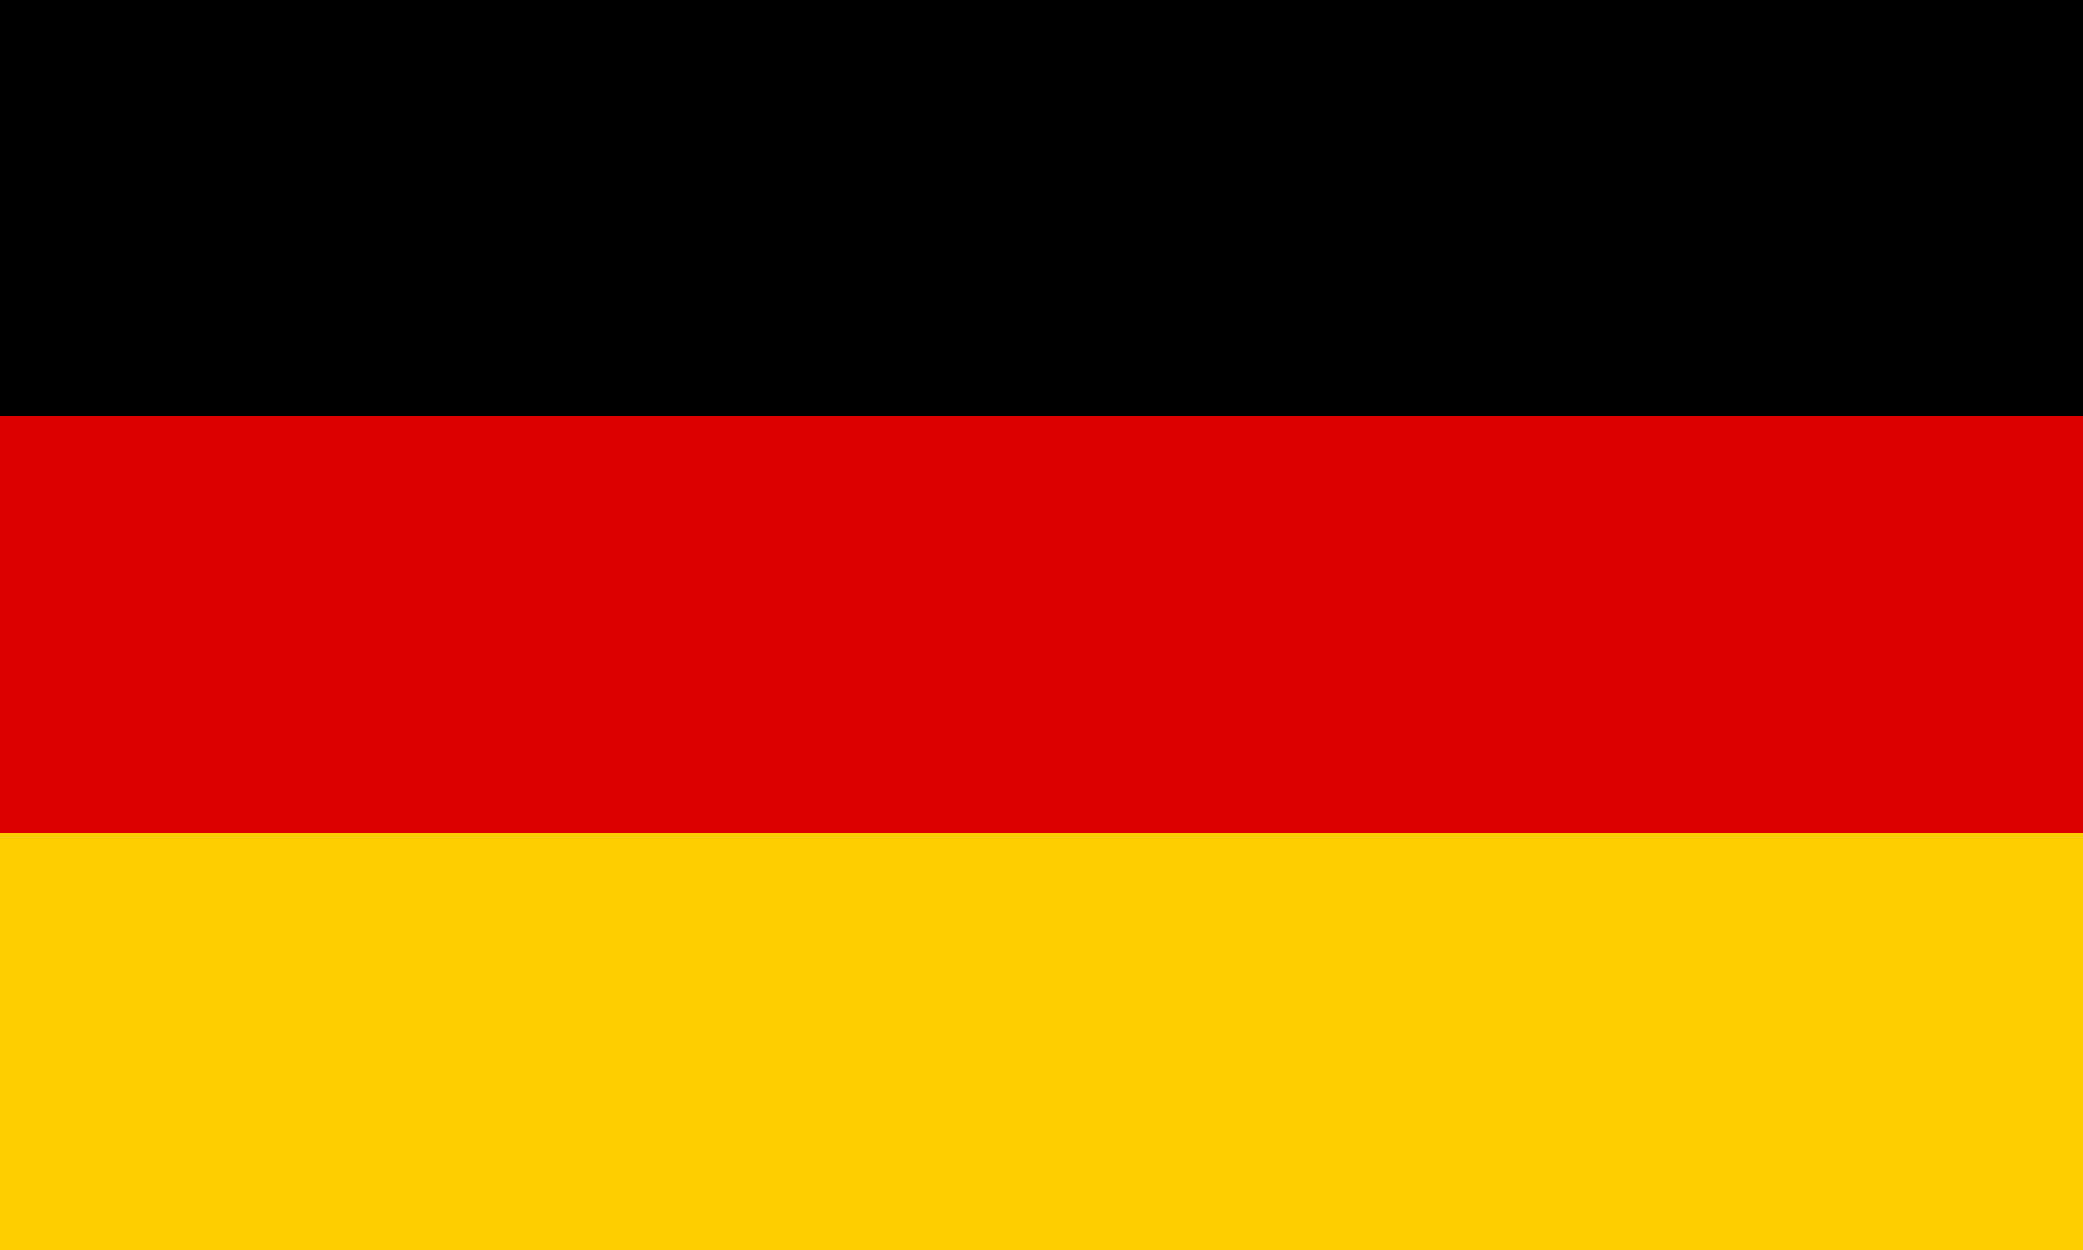
\includegraphics[width=1.0\linewidth]{Annexes/friseChronologique/img/Flag_of_Germany.pdf}
                \captionsetup{labelformat=empty}\refDrapeau{Drapeau Germany}{frise:Flag_of_Germany.pdf}
            \end{figure}
        \end{minipage}
    &
        \begin{minipage}{.65\textwidth}
            \textbf{1891} - \textbf{Premier vol en planeur}
            
            L'ingénieur allemand Otto Lilienthal fait voler son planeur, en se lancant depuis une colline
            \begin{figure}[H]
                \legende{L'un des vols d'Otto Lilienthal, ici en 1895}{frise:Otto_Lilienthal_gliding_experiment_ppmsca.02546.jpg}
            \end{figure}
        \end{minipage}
    &
        \begin{minipage}{.275\textwidth}
            \begin{figure}[H]
                \centering
                \includegraphics[width=1.0\linewidth]{Annexes/friseChronologique/img/Otto_Lilienthal_gliding_experiment_ppmsca.02546.jpg}
            \end{figure}
        \end{minipage}
    \end{tabular}
\end{table}
\begin{table}[H]
    \centering
    \begin{tabular}{c l c}
        \begin{minipage}{.075\textwidth}
            \begin{figure}[H]
            \setlength{\belowcaptionskip}{-40pt}
                \centering
                
\includegraphics[width=1.0\linewidth]{Annexes/friseChronologique/img/Flag_of_the_United_States_28DDD-F-416E_specifications29.pdf}
                \captionsetup{labelformat=empty}\refDrapeau{Drapeau the United States 28DDD-F-416E specifications29}{frise:Flag_of_the_United_States_28DDD-F-416E_specifications29.pdf}
            \end{figure}
        \end{minipage}
    &
        \begin{minipage}{.65\textwidth}
            \textbf{1896} - \textbf{Octave Chanute et le vol plané}
            
            L'ingénieur franco-américain Octave Chanute perfectionne les planeurs et effectue des centaines de vols. Ses travaux, notamment sur la structure biplan, influenceront directement les frères Wright. Il joue un rôle crucial dans la diffusion des connaissances aéronautiques.
            \begin{figure}[H]
                \legende{Planeur d'Octave Chanute en 1896}{frise:Chanute-Herring_1896_hang_glider.jpg}
            \end{figure}
        \end{minipage}
    &
        \begin{minipage}{.275\textwidth}
            \begin{figure}[H]
                \centering
                \includegraphics[width=1.0\linewidth]{Annexes/friseChronologique/img/Chanute-Herring_1896_hang_glider.jpg}
            \end{figure}
        \end{minipage}
    \end{tabular}
\end{table}
\begin{table}[H]
    \centering
    \begin{tabular}{c l c}
        \begin{minipage}{.075\textwidth}
            \begin{figure}[H]
            \setlength{\belowcaptionskip}{-40pt}
                \centering
                
\includegraphics[width=1.0\linewidth]{Annexes/friseChronologique/img/Flag_of_France.pdf}
                \captionsetup{labelformat=empty}\refDrapeau{Drapeau France}{frise:Flag_of_France.pdf}
            \end{figure}
        \end{minipage}
    &
        \begin{minipage}{.65\textwidth}
            \textbf{19 octobre 1901} - \textbf{Alberto Santos Dumont contourne la Tour Eiffel en dirigeable}
            
            En 1900, le mécène Henry Deutsch de la Meurthe crée une compétition, dotée de 100 000 francs, réservée aux seuls dirigeables et qui consiste à couvrir en moins de 30 minutes la distance entre Saint-Cloud et la tour Eiffel. Santos-Dumont y participe avec son dirigeable n°5. À sa première tentative, le 8 août 1901, il est victime d'un accident : alors qu'il a déjà viré la tour Eiffel, à la suite d'un dégonflement incontrôlable, son dirigeable heurte un immeuble au quai de Passy et il se retrouve suspendu au 5e étage ! Il réussit finalement le 19 octobre 1901 sur le n°6
            \begin{figure}[H]
                \legende{Internet Archive Book Images}{frise:Santos-Dumont_flight_around_the_Eiffel_Tower.jpg}
            \end{figure}
        \end{minipage}
    &
        \begin{minipage}{.275\textwidth}
            \begin{figure}[H]
                \centering
                \includegraphics[width=1.0\linewidth]{Annexes/friseChronologique/img/Santos-Dumont_flight_around_the_Eiffel_Tower.jpg}
            \end{figure}
        \end{minipage}
    \end{tabular}
\end{table}
\begin{table}[H]
    \centering
    \begin{tabular}{c l c}
        \begin{minipage}{.075\textwidth}
            \begin{figure}[H]
            \setlength{\belowcaptionskip}{-40pt}
                \centering
                
\includegraphics[width=1.0\linewidth]{Annexes/friseChronologique/img/Flag_of_the_United_States_28DDD-F-416E_specifications29.pdf}
                \captionsetup{labelformat=empty}\refDrapeau{Drapeau the United States 28DDD-F-416E specifications29}{frise:Flag_of_the_United_States_28DDD-F-416E_specifications29.pdf}
            \end{figure}
        \end{minipage}
    &
        \begin{minipage}{.65\textwidth}
            \textbf{1903} - \textbf{Premier vol d'un avion}
            
            Les frères Orville et Wilbur Wright font voler leur avion aux Etats-Unis.
Il s'agit du premier vol contrôlé d'un aérodyne motorisé
            \begin{figure}[H]
                \legende{Premier vol motorisé des frères Wright le 17 décembre 1903 sur Flyer.}{frise:Wrightflyer.jpg}
            \end{figure}
        \end{minipage}
    &
        \begin{minipage}{.275\textwidth}
            \begin{figure}[H]
                \centering
                \includegraphics[width=1.0\linewidth]{Annexes/friseChronologique/img/Wrightflyer.jpg}
            \end{figure}
        \end{minipage}
    \end{tabular}
\end{table}
\begin{table}[H]
    \centering
    \begin{tabular}{c l c}
        \begin{minipage}{.075\textwidth}
            \begin{figure}[H]
            \setlength{\belowcaptionskip}{-40pt}
                \centering
                
\includegraphics[width=1.0\linewidth]{Annexes/friseChronologique/img/Flag_of_France.pdf}
                \captionsetup{labelformat=empty}\refDrapeau{Drapeau France}{frise:Flag_of_France.pdf}
            \end{figure}
            
            \centering\mdiBrevet
        \end{minipage}
    &
        \begin{minipage}{.65\textwidth}
            \textbf{22 janvier 1907} - \textbf{Invention du manche à balai}
            
            Robert Esnault-Pelterie dépose le brevet pour le manche à balai, permettant de diriger les aéronefs
            \begin{figure}[H]
                \legende{Portrait de Robert Esnault-Pelterie}{frise:Robert_Esnault-Pelterie_1909.jpg}
            \end{figure}
        \end{minipage}
    &
        \begin{minipage}{.275\textwidth}
            \begin{figure}[H]
                \centering
                \includegraphics[width=1.0\linewidth]{Annexes/friseChronologique/img/Robert_Esnault-Pelterie_1909.jpg}
            \end{figure}
        \end{minipage}
    \end{tabular}
\end{table}
\begin{table}[H]
    \centering
    \begin{tabular}{c l c}
        \begin{minipage}{.075\textwidth}
            \begin{figure}[H]
            \setlength{\belowcaptionskip}{-40pt}
                \centering
                
\includegraphics[width=1.0\linewidth]{Annexes/friseChronologique/img/Flag_of_France.pdf}
                \captionsetup{labelformat=empty}\refDrapeau{Drapeau France}{frise:Flag_of_France.pdf}
            \end{figure}
            
            \centering\mdiFemale
        \end{minipage}
    &
        \begin{minipage}{.65\textwidth}
            \textbf{08 juillet 1908} - \textbf{Thérèse Peltier, première femme à quitter le sol}
            
            Le 8 juillet 1908, Thérèse Peltier devient la premier femme à quitter le sol avec un aéronef, dans un avion piloté par son compagnon Léon Delagrange.

Elle deviendra la première femme à voler seule à bord d'un avion quelque mois plus tard, lors de son lâcher solo.
            \begin{figure}[H]
                \legende{Thérèse Peltier à Issy-les-Moulineaux le 17 September 1908}{frise:ThC3A9rC3A8se_Peltier_1908.jpg}
            \end{figure}
        \end{minipage}
    &
        \begin{minipage}{.275\textwidth}
            \begin{figure}[H]
                \centering
                \includegraphics[width=1.0\linewidth]{Annexes/friseChronologique/img/ThC3A9rC3A8se_Peltier_1908.jpg}
            \end{figure}
        \end{minipage}
    \end{tabular}
\end{table}
\begin{table}[H]
    \centering
    \begin{tabular}{c l c}
        \begin{minipage}{.075\textwidth}
            \begin{figure}[H]
            \setlength{\belowcaptionskip}{-40pt}
                \centering
                
\includegraphics[width=1.0\linewidth]{Annexes/friseChronologique/img/Flag_of_France.pdf}
                \captionsetup{labelformat=empty}\refDrapeau{Drapeau France}{frise:Flag_of_France.pdf}
            \end{figure}
            
            \centering\mdiTrophy
        \end{minipage}
    &
        \begin{minipage}{.65\textwidth}
            \textbf{25 juillet 1909} - \textbf{Louis Blériot traverse la manche}
            
            "L'Angleterre n'est plus une île !" Le 25 juillet 1909, Louis Blériot relie Calais à Douvres à bord de son  Blériot XI.
            \begin{figure}[H]
                \legende{Blériot aux commandes de l'appareil de la traversée à la fête de Port-Aviation, le 4 juillet 1909.}{frise:Btv1b8433368f-p044_BlC3A9riot_C3A0_la_fC3AAte_de_Port-Aviation2C_dimanche_4_juillet_1909.jpg}
            \end{figure}
        \end{minipage}
    &
        \begin{minipage}{.275\textwidth}
            \begin{figure}[H]
                \centering
                \includegraphics[width=1.0\linewidth]{Annexes/friseChronologique/img/Btv1b8433368f-p044_BlC3A9riot_C3A0_la_fC3AAte_de_Port-Aviation2C_dimanche_4_juillet_1909.jpg}
            \end{figure}
        \end{minipage}
    \end{tabular}
\end{table}
\begin{table}[H]
    \centering
    \begin{tabular}{c l c}
        \begin{minipage}{.075\textwidth}
            \begin{figure}[H]
            \setlength{\belowcaptionskip}{-40pt}
                \centering
                
\includegraphics[width=1.0\linewidth]{Annexes/friseChronologique/img/Flag_of_France.pdf}
                \captionsetup{labelformat=empty}\refDrapeau{Drapeau France}{frise:Flag_of_France.pdf}
            \end{figure}
        \end{minipage}
    &
        \begin{minipage}{.65\textwidth}
            \textbf{07 octobre 1909} - \textbf{Louis Blériot obtient le premier brevet de pilote}
            
            Le brevet de pilote n°1 est délivré à Louis Blériot

Le 7 octobre 1909, l'Aéro-Club de France décide de décerner un brevet de pilote à seize pionniers de l'aviation. Personne n’osant faire passer un examen à ces pionniers, un comité prit la liste des pilotes et les classa par ordre alphabétique. Son nom commençant par un B, Louis Blériot se voit attribuer le brevet de pilote numéro 1. L’instauration du brevet de pilote intervient le 1er janvier 1910.
            \begin{figure}[H]
                \legende{Avant de délivrer des brevets de pilotes d'avion, l'Aéroclub de France délivrait également des brevets aux pilotes de ballons. Brevet de pilote aéronaute décerné par l'Aéro-Club de France à Paul Tissandier (1904).}{frise:Brevet_de_pilote_aC3A9ronaute_1904.jpg}
            \end{figure}
        \end{minipage}
    &
        \begin{minipage}{.275\textwidth}
            \begin{figure}[H]
                \centering
                \includegraphics[width=1.0\linewidth]{Annexes/friseChronologique/img/Brevet_de_pilote_aC3A9ronaute_1904.jpg}
            \end{figure}
        \end{minipage}
    \end{tabular}
\end{table}
\begin{table}[H]
    \centering
    \begin{tabular}{c l c}
        \begin{minipage}{.075\textwidth}
            \begin{figure}[H]
            \setlength{\belowcaptionskip}{-40pt}
                \centering
                
\includegraphics[width=1.0\linewidth]{Annexes/friseChronologique/img/Flag_of_France.pdf}
                \captionsetup{labelformat=empty}\refDrapeau{Drapeau France}{frise:Flag_of_France.pdf}
            \end{figure}
            
            \centering\mdiFemale
        \end{minipage}
    &
        \begin{minipage}{.65\textwidth}
            \textbf{08 mars 1910} - \textbf{Élisa Deroche, première femme brevetée pilote}
            
            Élisa Deroche s'interesse à l'aviation depuis l'année 1906.
Fin 1909, elle effectue son premier vol solo, et son brevet (le n°36) lui sera délivré quelques mois plus tard, le 8 mars 1910.

La semaine internationale des femmes de l'air marque désormais chaque année cette date historique, puisque cette semaine est positionnée sur la semaine du 8 mars. 

            \begin{figure}[H]
                \legende{Elise Deroche aux commandes d'un biplan Voisin.}{frise:Les_Maitres_de_l27aviation._Mme._la_Baronne_de_Laroche2C_aviatrice2C_au_poste_de_direction_d27un_biplan_Voisin._cph.3c07402.jpg}
            \end{figure}
        \end{minipage}
    &
        \begin{minipage}{.275\textwidth}
            \begin{figure}[H]
                \centering
                \includegraphics[width=1.0\linewidth]{Annexes/friseChronologique/img/Les_Maitres_de_l27aviation._Mme._la_Baronne_de_Laroche2C_aviatrice2C_au_poste_de_direction_d27un_biplan_Voisin._cph.3c07402.jpg}
            \end{figure}
        \end{minipage}
    \end{tabular}
\end{table}
\begin{table}[H]
    \centering
    \begin{tabular}{c l c}
        \begin{minipage}{.075\textwidth}
            \begin{figure}[H]
            \setlength{\belowcaptionskip}{-40pt}
                \centering
                
\includegraphics[width=1.0\linewidth]{Annexes/friseChronologique/img/Flag_of_France.pdf}
                \captionsetup{labelformat=empty}\refDrapeau{Drapeau France}{frise:Flag_of_France.pdf}
            \end{figure}
        \end{minipage}
    &
        \begin{minipage}{.65\textwidth}
            \textbf{28 mars 1910} - \textbf{Premier vol d'un hydravion}
            
            L'ingénieur français Henri Fabre devient le premier à décoller d'un plan d'eau avec un aéronef qui dispose de son propre moyen de propulsion. Cette date marque l'entrée dans l'ère de l'hydraviation qui aura son âge d'or sur la période de l'entre 2 guerres.
            \begin{figure}[H]
                \legende{Hydroplane d'Henri Fabre}{frise:Hydroplane_28de_Henri29_Fabre_28Monaco2C_concours_de_canots_automobiles2C_2_-17_avril29_1911_-_btv1b53240713d.jpg}
            \end{figure}
        \end{minipage}
    &
        \begin{minipage}{.275\textwidth}
            \begin{figure}[H]
                \centering
                \includegraphics[width=1.0\linewidth]{Annexes/friseChronologique/img/Hydroplane_28de_Henri29_Fabre_28Monaco2C_concours_de_canots_automobiles2C_2_-17_avril29_1911_-_btv1b53240713d.jpg}
            \end{figure}
        \end{minipage}
    \end{tabular}
\end{table}
\begin{table}[H]
    \centering
    \begin{tabular}{c l c}
        \begin{minipage}{.075\textwidth}
            \begin{figure}[H]
            \setlength{\belowcaptionskip}{-40pt}
                \centering
                
\includegraphics[width=1.0\linewidth]{Annexes/friseChronologique/img/Flag_of_France.pdf}
                \captionsetup{labelformat=empty}\refDrapeau{Drapeau France}{frise:Flag_of_France.pdf}
            \end{figure}
            
            \centering\mdiBrevet
        \end{minipage}
    &
        \begin{minipage}{.65\textwidth}
            \textbf{1911} - \textbf{Raoul Badin invente l'anémomètre}
            
            L'inventeur français invente un dispositif permettant la mesure de la vitesse de l'air dans lequel évolue un aéronef. L'anémomère est parfois appelé "badin" du nom de cet inventeur
            \begin{figure}[H]
                \legende{Illustration d'un anémomètre moderne}{frise:Airspeed_indicator.pdf}
            \end{figure}
        \end{minipage}
    &
        \begin{minipage}{.275\textwidth}
            \begin{figure}[H]
                \centering
                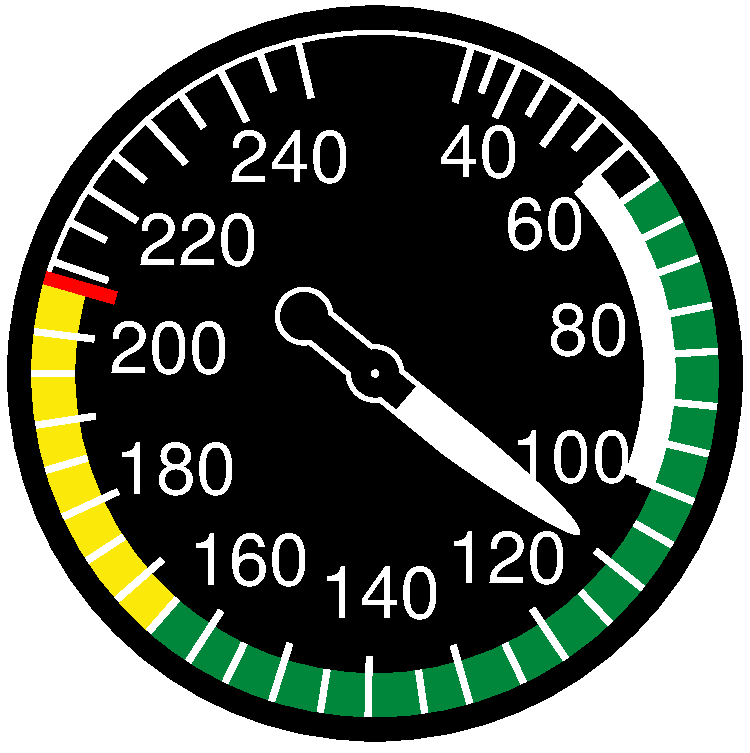
\includegraphics[width=1.0\linewidth]{Annexes/friseChronologique/img/Airspeed_indicator.pdf}
            \end{figure}
        \end{minipage}
    \end{tabular}
\end{table}
\begin{table}[H]
    \centering
    \begin{tabular}{c l c}
        \begin{minipage}{.075\textwidth}
            \begin{figure}[H]
            \setlength{\belowcaptionskip}{-40pt}
                \centering
                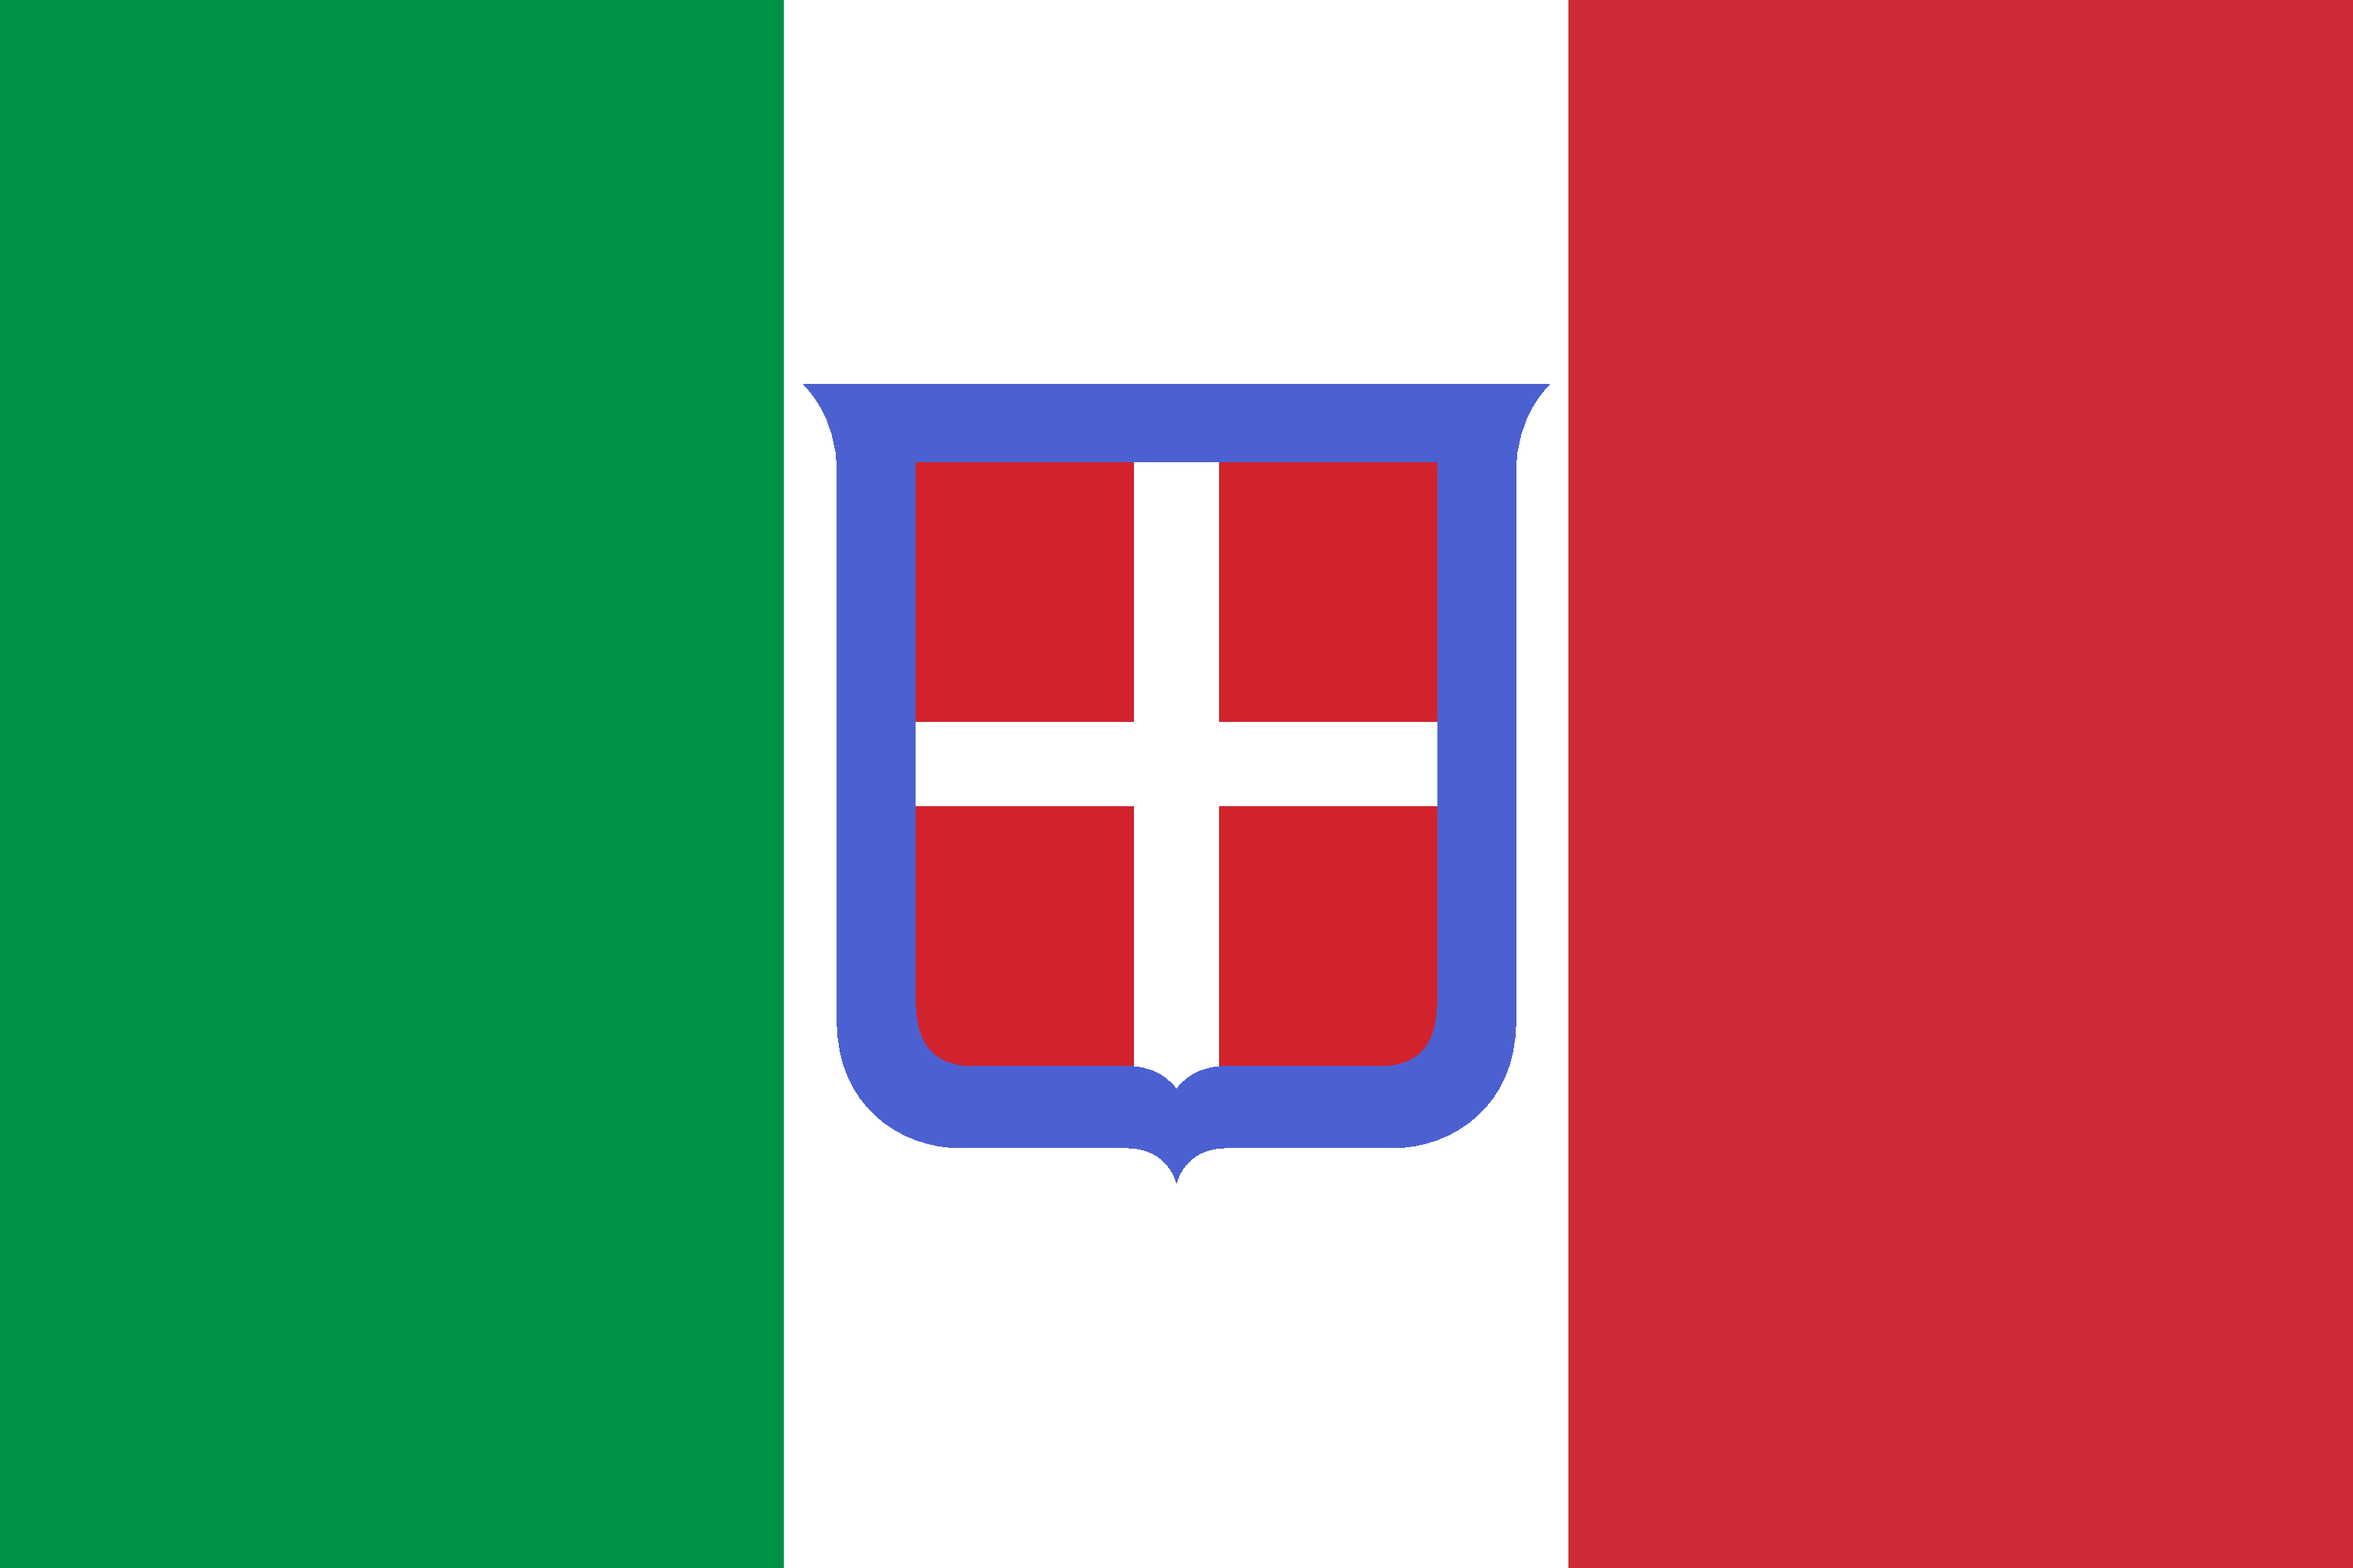
\includegraphics[width=1.0\linewidth]{Annexes/friseChronologique/img/Flag_of_Italy_281861E28093194629.pdf}
                \captionsetup{labelformat=empty}\refDrapeau{Drapeau Italy 281861E28093194629}{frise:Flag_of_Italy_281861E28093194629.pdf}
            \end{figure}
            
            \centering\mdiMilitaire
        \end{minipage}
    &
        \begin{minipage}{.65\textwidth}
            \textbf{23 novembre 1911} - \textbf{Premier usage d'avions au combat}
            
            Les Italiens sont les premiers à utiliser des avions au combat à l'occasion de la guerre de Libye.

Les Italiens utilisent des avions Blériot XI, Nieuport, Farman et Etrich Taube
            \begin{figure}[H]
                \legende{Avion italien lors d'un attaque en Libye}{frise:Italian_Nieuport_IV_attacking_Ottoman_forces_in_Libya_1911_or_1912.jpg}
            \end{figure}
        \end{minipage}
    &
        \begin{minipage}{.275\textwidth}
            \begin{figure}[H]
                \centering
                \includegraphics[width=1.0\linewidth]{Annexes/friseChronologique/img/Italian_Nieuport_IV_attacking_Ottoman_forces_in_Libya_1911_or_1912.jpg}
            \end{figure}
        \end{minipage}
    \end{tabular}
\end{table}
\begin{table}[H]
    \centering
    \begin{tabular}{c l c}
        \begin{minipage}{.075\textwidth}
            \begin{figure}[H]
            \setlength{\belowcaptionskip}{-40pt}
                \centering
                \includegraphics[width=1.0\linewidth]{Annexes/friseChronologique/img/Flag_of_France.pdf}
                \captionsetup{labelformat=empty}\refDrapeau{Drapeau France}{frise:Flag_of_France.pdf}
            \end{figure}
        \end{minipage}
    &
        \begin{minipage}{.65\textwidth}
            \textbf{21 septembre 1913} - \textbf{Adolphe Pégoud : premier looping}
            
            Le 19 août 1913, Adolphe Pegoud est le premier pilote de l'histoire à utiliser un parachute pour abandonner un avion en perdition.

L'histoire raconte que l'avion qu'il venait de quitter aurait alors effecuté un looping. C'est de cet événément qu'Adolphe Pegoud aurait tiré l'idée de réaliser un looping à bord de son avion, chose qu'il réalise le 21 septembre.
            \begin{figure}[H]
                \legende{Carte postale allemande illustrant le looping d'Adolphe Pegoud.}{frise:Adolphe_PC3A9goud_Looping.jpg}
            \end{figure}
        \end{minipage}
    &
        \begin{minipage}{.275\textwidth}
            \begin{figure}[H]
                \centering
                \includegraphics[width=1.0\linewidth]{Annexes/friseChronologique/img/Adolphe_PC3A9goud_Looping.jpg}
            \end{figure}
        \end{minipage}
    \end{tabular}
\end{table}
\begin{table}[H]
    \centering
    \begin{tabular}{c l c}
        \begin{minipage}{.075\textwidth}
            \begin{figure}[H]
            \setlength{\belowcaptionskip}{-40pt}
                \centering
                \includegraphics[width=1.0\linewidth]{Annexes/friseChronologique/img/Flag_of_France.pdf}
                \captionsetup{labelformat=empty}\refDrapeau{Drapeau France}{frise:Flag_of_France.pdf}
            \end{figure}
            
            \centering\mdiTrophy
        \end{minipage}
    &
        \begin{minipage}{.65\textwidth}
            \textbf{23 septembre 1913} - \textbf{Roland Garros traverse la Méditerranée}
            
            Roland Garros devient célèbre en réalisant la première traversée de la Méditerranée en avion, reliant Fréjus (France) à Bizerte (Tunisie) en 7h53 à bord d'un Morane-Saulnier.
            \begin{figure}[H]
                \legende{Roland Garros devant un avion Demoiselle B.C. (1910)}{frise:Roland_Garros_1910.jpg}
            \end{figure}
        \end{minipage}
    &
        \begin{minipage}{.275\textwidth}
            \begin{figure}[H]
                \centering
                \includegraphics[width=1.0\linewidth]{Annexes/friseChronologique/img/Roland_Garros_1910.jpg}
            \end{figure}
        \end{minipage}
    \end{tabular}
\end{table}
\section{La première guerre mondiale}
La Grande Guerre transforme radicalement l'aviation. D'abord utilisés pour l'observation depuis des ballons captifs (les "saucisses") ou des avions de reconnaissance, les aéronefs deviennent rapidement des armes de combat. L'innovation s'accélère : synchronisation du tir à travers l'hélice, pilote automatique de Sperry, amélioration des performances (la vitesse moyenne est multipliée par 2). Des as légendaires émergent : Georges Guynemer, René Fonck (l'as des as français avec 75 victoires), Manfred von Richthofen (le Baron Rouge avec 80 victoires), Max Immelmann qui donne son nom à une manœuvre acrobatique. Marcel Bloch (futur Dassault) conçoit l'hélice Éclair qui équipera les meilleurs chasseurs français. La guerre aérienne change la nature même des conflits, ajoutant une troisième dimension au champ de bataille.
\begin{table}[H]
    \centering
    \begin{tabular}{c l c}
        \begin{minipage}{.075\textwidth}
            \begin{figure}[H]
            \setlength{\belowcaptionskip}{-40pt}
                \centering
                \includegraphics[width=1.0\linewidth]{Annexes/friseChronologique/img/Flag_of_the_United_States_28DDD-F-416E_specifications29.pdf}
                \captionsetup{labelformat=empty}\refDrapeau{Drapeau the United States 28DDD-F-416E specifications29}{frise:Flag_of_the_United_States_28DDD-F-416E_specifications29.pdf}
            \end{figure}
            
            \centering\mdiBrevet
        \end{minipage}
    &
        \begin{minipage}{.65\textwidth}
            \textbf{1914} - \textbf{Lawrence Sperry invente le pilote automatique}
            
            En 1914, l'ingénieur américain Lawrence Sperry développe le premier pilote automatique gyroscopique, permettant à un avion de maintenir automatiquement son cap et son assiette. Cette innovation révolutionnera l'aviation.
            \begin{figure}[H]
                \legende{Lawrence Sperry}{frise:LawrenceSperry.jpg}
            \end{figure}
        \end{minipage}
    &
        \begin{minipage}{.275\textwidth}
            \begin{figure}[H]
                \centering
                \includegraphics[width=1.0\linewidth]{Annexes/friseChronologique/img/LawrenceSperry.jpg}
            \end{figure}
        \end{minipage}
    \end{tabular}
\end{table}
\begin{table}[H]
    \centering
    \begin{tabular}{c l c}
        \begin{minipage}{.075\textwidth}
            \begin{figure}[H]
            \setlength{\belowcaptionskip}{-40pt}
                \centering
                \includegraphics[width=1.0\linewidth]{Annexes/friseChronologique/img/Flag_of_Germany.pdf}
                \captionsetup{labelformat=empty}\refDrapeau{Drapeau Germany}{frise:Flag_of_Germany.pdf}
            \end{figure}
            
            \centering\mdiMilitaire
        \end{minipage}
    &
        \begin{minipage}{.65\textwidth}
            \textbf{1915} - \textbf{Max Immelmann et sa manœuvre}
            
            L'as allemand Max Immelmann donne son nom à une manœuvre acrobatique permettant d'inverser rapidement la direction du vol : le "retournement Immelmann". Cette figure combine un demi-looping suivi d'un demi-tonneau.
            \begin{figure}[H]
                \legende{Illustration de la manoeuvre de l'Immelmann}{frise:Immelmann_turn.pdf}
            \end{figure}
        \end{minipage}
    &
        \begin{minipage}{.275\textwidth}
            \begin{figure}[H]
                \centering
                \includegraphics[width=1.0\linewidth]{Annexes/friseChronologique/img/Immelmann_turn.pdf}
            \end{figure}
        \end{minipage}
    \end{tabular}
\end{table}
\begin{table}[H]
    \centering
    \begin{tabular}{c l c}
        \begin{minipage}{.075\textwidth}
            \begin{figure}[H]
            \setlength{\belowcaptionskip}{-40pt}
                \centering
                \includegraphics[width=1.0\linewidth]{Annexes/friseChronologique/img/International_Flag_of_Planet_Earth.pdf}
                \captionsetup{labelformat=empty}\refDrapeau{International Drapeau Planet Earth}{frise:International_Flag_of_Planet_Earth.pdf}
            \end{figure}
            
            \centering\mdiMilitaire
        \end{minipage}
    &
        \begin{minipage}{.65\textwidth}
            \textbf{1914} - \textbf{Ballons captifs d'observation, les "saucisses"}
            
            Durant la Première Guerre mondiale, les armées utilisent massivement des ballons captifs pour observer les mouvements ennemis. Ces ballons sont familièrement appelés "saucisses" en raison de leur forme allongée.
            \begin{figure}[H]
                \legende{Ballon d'observation allemand Parseval-Siegsfeld}{frise:Balloons_28WWI29.jpg}
            \end{figure}
        \end{minipage}
    &
        \begin{minipage}{.275\textwidth}
            \begin{figure}[H]
                \centering
                \includegraphics[width=1.0\linewidth]{Annexes/friseChronologique/img/Balloons_28WWI29.jpg}
            \end{figure}
        \end{minipage}
    \end{tabular}
\end{table}
\begin{table}[H]
    \centering
    \begin{tabular}{c l c}
        \begin{minipage}{.075\textwidth}
            \begin{figure}[H]
            \setlength{\belowcaptionskip}{-40pt}
                \centering
                \includegraphics[width=1.0\linewidth]{Annexes/friseChronologique/img/Flag_of_France.pdf}
                \captionsetup{labelformat=empty}\refDrapeau{Drapeau France}{frise:Flag_of_France.pdf}
            \end{figure}
            
            \centering\mdiMilitaire
        \end{minipage}
    &
        \begin{minipage}{.65\textwidth}
            \textbf{1914} - \textbf{René Fonck, as des as}
            
            René Fonck est le pilote français ayant le plus grand nombre de victoires aériennes (75). Il est surnomé "l'as des as"
            \begin{figure}[H]
                \legende{Portrait de René Fonck}{frise:RenC3A9_Fonck_02.jpg}
            \end{figure}
        \end{minipage}
    &
        \begin{minipage}{.275\textwidth}
            \begin{figure}[H]
                \centering
                \includegraphics[width=1.0\linewidth]{Annexes/friseChronologique/img/RenC3A9_Fonck_02.jpg}
            \end{figure}
        \end{minipage}
    \end{tabular}
\end{table}
\begin{table}[H]
    \centering
    \begin{tabular}{c l c}
        \begin{minipage}{.075\textwidth}
            \begin{figure}[H]
            \setlength{\belowcaptionskip}{-40pt}
                \centering
                \includegraphics[width=1.0\linewidth]{Annexes/friseChronologique/img/Flag_of_Germany.pdf}
                \captionsetup{labelformat=empty}\refDrapeau{Drapeau Germany}{frise:Flag_of_Germany.pdf}
            \end{figure}
            
            \centering\mdiMilitaire
        \end{minipage}
    &
        \begin{minipage}{.65\textwidth}
            \textbf{1914} - \textbf{Manfred von Richtoffen, as de la première guerre mondiale}
            
            Manfred von Richtoffen, pilote allemand, dispose du plus grand nombre de victoires confirmées (80) lors du premier conflit mondial.

Il est connu sous le nom du Baron rouge
            \begin{figure}[H]
                \legende{Le Baron Rouge, Manfred von Richtoffen}{frise:Manfred_von_Richthofen.jpg}
            \end{figure}
        \end{minipage}
    &
        \begin{minipage}{.275\textwidth}
            \begin{figure}[H]
                \centering
                \includegraphics[width=1.0\linewidth]{Annexes/friseChronologique/img/Manfred_von_Richthofen.jpg}
            \end{figure}
        \end{minipage}
    \end{tabular}
\end{table}
\begin{table}[H]
    \centering
    \begin{tabular}{c l c}
        \begin{minipage}{.075\textwidth}
            \begin{figure}[H]
            \setlength{\belowcaptionskip}{-40pt}
                \centering
                \includegraphics[width=1.0\linewidth]{Annexes/friseChronologique/img/Flag_of_Germany.pdf}
                \captionsetup{labelformat=empty}\refDrapeau{Drapeau Germany}{frise:Flag_of_Germany.pdf}
            \end{figure}
        \end{minipage}
    &
        \begin{minipage}{.65\textwidth}
            \textbf{12 décembre 1915} - \textbf{Premier vol du Junker J1, premier avion entièrement métallique}
            
            Hugo Junkers avec ses 15 collaborateurs et malgré les techniques de soudage non encore parfaitement au point, réussit à faire voler ce nouveau concept révolutionnaire le 12 décembre 1915 après seulement 3 mois de fabrication.

Le J 1, dont le revêtement était constitué de tôles d'acier de 0,1 à 0,2 mm d'épaisseur était cependant trop lourd (masse à vide de 937 kg contre seulement 400 kg pour le Fokker E.III) et il ne fut pas commandé en série par les services officiels.
            \begin{figure}[H]
                \legende{Junker J1}{frise:Junkers_J_1_at_DC3B6beritz_1915.jpg}
            \end{figure}
        \end{minipage}
    &
        \begin{minipage}{.275\textwidth}
            \begin{figure}[H]
                \centering
                \includegraphics[width=1.0\linewidth]{Annexes/friseChronologique/img/Junkers_J_1_at_DC3B6beritz_1915.jpg}
            \end{figure}
        \end{minipage}
    \end{tabular}
\end{table}
\begin{table}[H]
    \centering
    \begin{tabular}{c l c}
        \begin{minipage}{.075\textwidth}
            \begin{figure}[H]
            \setlength{\belowcaptionskip}{-40pt}
                \centering
                \includegraphics[width=1.0\linewidth]{Annexes/friseChronologique/img/Flag_of_France.pdf}
                \captionsetup{labelformat=empty}\refDrapeau{Drapeau France}{frise:Flag_of_France.pdf}
            \end{figure}
            
            \centering\mdiBrevet
        \end{minipage}
    &
        \begin{minipage}{.65\textwidth}
            \textbf{01 février 1916} - \textbf{Marcel Bloch concoit l'hélice Éclair}
            
            Marcel Dassault (qui s'appelait alors Marcel Bloch) dessine l'hélice Éclair. Cette hélice à marqué l'histoire car elle est très performante. Elle sera produite à plus de 4000 exemplaire et montée sur 10 des 20 avions les plus perfomants de l'armée française de cette époque.
            \begin{figure}[H]
                \legende{Le SPAD VII de Georges Guynemer, équipé de l'hélice Eclair}{frise:Georges_Guynemer27s_SPAD_VII2C_Musee_de_l27Air_et_de_l27Espace2C_Le_Bourget2C_Paris._28812284872329.jpg}
            \end{figure}
        \end{minipage}
    &
        \begin{minipage}{.275\textwidth}
            \begin{figure}[H]
                \centering
                \includegraphics[width=1.0\linewidth]{Annexes/friseChronologique/img/Georges_Guynemer27s_SPAD_VII2C_Musee_de_l27Air_et_de_l27Espace2C_Le_Bourget2C_Paris._28812284872329.jpg}
            \end{figure}
        \end{minipage}
    \end{tabular}
\end{table}
\section{L'entre 2 guerres}
L'entre-deux-guerres est l'âge d'or de l'aviation pionnière. Georges Latécoère fonde l'Aéropostale en 1918, créant des lignes vers l'Afrique et l'Amérique du Sud avec des pilotes légendaires comme Mermoz, Guillaumet et Saint-Exupéry. Les exploits se multiplient : Lindbergh traverse l'Atlantique en 1927, Costes et Bellonte réalisent Paris-New York en 1930. Les femmes s'illustrent : Adrienne Bolland franchit les Andes en 1921, Maryse Bastié traverse l'Atlantique Sud en 1936, Amelia Earhart devient une icône. L'aviation commerciale se structure avec la création d'Air France en 1933 et l'essor des hydravions à Biscarosse. Le DC-3 Dakota révolutionne le transport aérien. Pendant ce temps, interdite d'aviation militaire motorisée, l'Allemagne devient leader mondial du vol à voile, formant secrètement de futurs pilotes. Les innovations techniques se poursuivent : autogire, hélicoptère de Cornu, instruments...
\begin{table}[H]
    \centering
    \begin{tabular}{c l c}
        \begin{minipage}{.075\textwidth}
            \begin{figure}[H]
            \setlength{\belowcaptionskip}{-40pt}
                \centering
                \includegraphics[width=1.0\linewidth]{Annexes/friseChronologique/img/Flag_of_France.pdf}
                \captionsetup{labelformat=empty}\refDrapeau{Drapeau France}{frise:Flag_of_France.pdf}
            \end{figure}
        \end{minipage}
    &
        \begin{minipage}{.65\textwidth}
            \textbf{25 décembre 1918} - \textbf{Georges Latécoère lance l'Aéropostale}
            
            L'Aéropostale est le transport de courrier et frets (colis) par voie aérienne.

Le 25 décembre 1918, il ouvre la ligne entre Toulouse et Barcelone.

Dès 1919, la ligne est étendue jusqu'à Casablanca. Elle sera par la suite prolongée jusqu'à Dakar puis l'Amérique du Sud via Rio au Brésil, puis jusqu'à Buenos-Aires et Santiago du Chili
            \begin{figure}[H]
                \legende{Carte illustrant les lignes de l'aéropostale entre la France et l'Amérique du Sud, en 1930.}{frise:AC3A9ropostale._AmC3A9rique_du_Sud._Maroc_-_AlgC3A9rie_-_Afrique_Occidentale_FranC3A7aise_-_affiche_-_btv1b10104627j.jpg}
            \end{figure}
        \end{minipage}
    &
        \begin{minipage}{.275\textwidth}
            \begin{figure}[H]
                \centering
                \includegraphics[width=1.0\linewidth]{Annexes/friseChronologique/img/AC3A9ropostale._AmC3A9rique_du_Sud._Maroc_-_AlgC3A9rie_-_Afrique_Occidentale_FranC3A7aise_-_affiche_-_btv1b10104627j.jpg}
            \end{figure}
        \end{minipage}
    \end{tabular}
\end{table}
\begin{table}[H]
    \centering
    \begin{tabular}{c l c}
        \begin{minipage}{.075\textwidth}
            \begin{figure}[H]
            \setlength{\belowcaptionskip}{-40pt}
                \centering
                \includegraphics[width=1.0\linewidth]{Annexes/friseChronologique/img/Flag_of_France.pdf}
                \captionsetup{labelformat=empty}\refDrapeau{Drapeau France}{frise:Flag_of_France.pdf}
            \end{figure}
            
            \centering\mdiFemale
            
            \centering\mdiTrophy
        \end{minipage}
    &
        \begin{minipage}{.65\textwidth}
            \textbf{01 avril 1921} - \textbf{Adrienne Bolland, première femme à traverser la Cordillière des Andes}
            
            Adrienne Bolland traverse la Cordillière en Caudron G3 en 4h15
            \begin{figure}[H]
                \legende{Adrienne Bolland faisant la couverture du magazine argentin El Gráfico le 19 mars 1921}{frise:Adrienne_Bolland_-_El_GrC3A1fico_91.jpg}
            \end{figure}
        \end{minipage}
    &
        \begin{minipage}{.275\textwidth}
            \begin{figure}[H]
                \centering
                \includegraphics[width=1.0\linewidth]{Annexes/friseChronologique/img/Adrienne_Bolland_-_El_GrC3A1fico_91.jpg}
            \end{figure}
        \end{minipage}
    \end{tabular}
\end{table}
\begin{table}[H]
    \centering
    \begin{tabular}{c l c}
        \begin{minipage}{.075\textwidth}
            \begin{figure}[H]
            \setlength{\belowcaptionskip}{-40pt}
                \centering
                \includegraphics[width=1.0\linewidth]{Annexes/friseChronologique/img/Flag_of_Spain.pdf}
                \captionsetup{labelformat=empty}\refDrapeau{Drapeau Spain}{frise:Flag_of_Spain.pdf}
            \end{figure}
        \end{minipage}
    &
        \begin{minipage}{.65\textwidth}
            \textbf{1923} - \textbf{Premier vol d'un autogire}
            
            Juan de la Cierva effectue le premier vol d'un autogire
            \begin{figure}[H]
                \legende{L'autogire C-6 de Juan de la Cierva (1925)}{frise:Autogyro_at_Farnborough2C_1925_28Our_Generation2C_193829.jpg}
            \end{figure}
        \end{minipage}
    &
        \begin{minipage}{.275\textwidth}
            \begin{figure}[H]
                \centering
                \includegraphics[width=1.0\linewidth]{Annexes/friseChronologique/img/Autogyro_at_Farnborough2C_1925_28Our_Generation2C_193829.jpg}
            \end{figure}
        \end{minipage}
    \end{tabular}
\end{table}
\begin{table}[H]
    \centering
    \begin{tabular}{c l c}
        \begin{minipage}{.075\textwidth}
            \begin{figure}[H]
            \setlength{\belowcaptionskip}{-40pt}
                \centering
                \includegraphics[width=1.0\linewidth]{Annexes/friseChronologique/img/Flag_of_the_United_States_28DDD-F-416E_specifications29.pdf}
                \captionsetup{labelformat=empty}\refDrapeau{Drapeau the United States 28DDD-F-416E specifications29}{frise:Flag_of_the_United_States_28DDD-F-416E_specifications29.pdf}
            \end{figure}
            
            \centering\mdiTrophy
        \end{minipage}
    &
        \begin{minipage}{.65\textwidth}
            \textbf{20 mai 1927} - \textbf{Charles Lindbergh réalise le premier vol transaltantique }
            
            Charles Lindbergh réalise le premier vol transaltantique entre New-York et Paris, à bord de son avion,  le Spirit of Saint-Louis
            \begin{figure}[H]
                \legende{}{frise:Col_Charles_Lindbergh2C_original2C_hec.21329.jpg}
            \end{figure}
        \end{minipage}
    &
        \begin{minipage}{.275\textwidth}
            \begin{figure}[H]
                \centering
                \includegraphics[width=1.0\linewidth]{Annexes/friseChronologique/img/Col_Charles_Lindbergh2C_original2C_hec.21329.jpg}
            \end{figure}
        \end{minipage}
    \end{tabular}
\end{table}
\begin{table}[H]
    \centering
    \begin{tabular}{c l c}
        \begin{minipage}{.075\textwidth}
            \begin{figure}[H]
            \setlength{\belowcaptionskip}{-40pt}
                \centering
                \includegraphics[width=1.0\linewidth]{Annexes/friseChronologique/img/Flag_of_France.pdf}
                \captionsetup{labelformat=empty}\refDrapeau{Drapeau France}{frise:Flag_of_France.pdf}
            \end{figure}
            
            \centering\mdiFemale
            
            \centering\faTrophy
        \end{minipage}
    &
        \begin{minipage}{.65\textwidth}
            \textbf{13 juillet 1928} - \textbf{Maryse Bastié, première recordwomen de distance}
            
            Elle fut la première aviatrice française à accrocher de nombreux records féminins d'aviation à son palmarès. Ses exploits furent très rapidement médiatisés.

Le 13 juillet 1928, elle établit un premier record féminin homologué de distance (1 058 km), entre Paris et Treptow-sur-Rega, en Poméranie occidentale.

En 1929, elle établit un nouveau record de France féminin de durée de vol, de 10 h 30, et un record international féminin de durée avec 26 h 44. Ce record lui est repris le 2 mai 1930 par Léna Bernstein (35 h 45). Bien décidée à le récupérer, elle fait décoller son avion, un Klemm L 25 à moteur Salmson et modifié, le soir du 2 septembre 1930 et se pose le surlendemain après 37 h 55 de vol. Elle a lutté jusqu'à l'épuisement contre le froid et le manque de sommeil. Elle établit ensuite un record de distance avec 2 976 km sur le parcours Paris - Uhring (URSS). Pour cet exploit, à son retour, elle reçoit la croix de chevalier de la Légion d'honneur et le Harmon Trophy américain décerné, pour la première fois, à une Française.
            \begin{figure}[H]
                \legende{L'aviatrice française Maryse Bastié à ses débuts.}{frise:Maryse_bastie.jpg}
            \end{figure}
        \end{minipage}
    &
        \begin{minipage}{.275\textwidth}
            \begin{figure}[H]
                \centering
                \includegraphics[width=1.0\linewidth]{Annexes/friseChronologique/img/Maryse_bastie.jpg}
            \end{figure}
        \end{minipage}
    \end{tabular}
\end{table}
\begin{table}[H]
    \centering
    \begin{tabular}{c l c}
        \begin{minipage}{.075\textwidth}
            \begin{figure}[H]
            \setlength{\belowcaptionskip}{-40pt}
                \centering
                \includegraphics[width=1.0\linewidth]{Annexes/friseChronologique/img/Flag_of_France.pdf}
                \captionsetup{labelformat=empty}\refDrapeau{Drapeau France}{frise:Flag_of_France.pdf}
            \end{figure}
            
            \centering\mdiTrophy
        \end{minipage}
    &
        \begin{minipage}{.65\textwidth}
            \textbf{12 mai 1930} - \textbf{Jean Mermoz traverse l'Atlantique Sud}
            
            Jean Mermoz, pilote légendaire de l'Aéropostale, réalise la première traversée postale de l'Atlantique Sud entre Dakar et Natal (Brésil) à bord du Latécoère 28 "Comte de la Vaulx", ouvrant ainsi la voie aérienne vers l'Amérique du Sud.
            \begin{figure}[H]
                \legende{Le Croix du Sud, avion a bord duquel Jean Mermoz disparaîtra en mer en 1936}{frise:LatC3A9coere_300_Croix-du-Sud.jpg}
            \end{figure}
        \end{minipage}
    &
        \begin{minipage}{.275\textwidth}
            \begin{figure}[H]
                \centering
                \includegraphics[width=1.0\linewidth]{Annexes/friseChronologique/img/LatC3A9coere_300_Croix-du-Sud.jpg}
            \end{figure}
        \end{minipage}
    \end{tabular}
\end{table}
\begin{table}[H]
    \centering
    \begin{tabular}{c l c}
        \begin{minipage}{.075\textwidth}
            \begin{figure}[H]
            \setlength{\belowcaptionskip}{-40pt}
                \centering
                \includegraphics[width=1.0\linewidth]{Annexes/friseChronologique/img/Flag_of_France.pdf}
                \captionsetup{labelformat=empty}\refDrapeau{Drapeau France}{frise:Flag_of_France.pdf}
            \end{figure}
            
            \centering\mdiTrophy
        \end{minipage}
    &
        \begin{minipage}{.65\textwidth}
            \textbf{02 septembre 1930} - \textbf{Costes et Bellonte : première traversée Paris-New York}
            
            Les aviateurs français Dieudonné Costes et Maurice Bellonte réalisent la première traversée de l'Atlantique Nord dans le sens difficile (d'Est en Ouest, contre les vents dominants) à bord du Breguet 19 "Point d'Interrogation", reliant Le Bourget à New York.
            \begin{figure}[H]
                \legende{Le Point d'Interrogation au musée du Bourget}{frise:Point_d27interrogation_Musee_du_Bourget_P1010705.JPG}
            \end{figure}
        \end{minipage}
    &
        \begin{minipage}{.275\textwidth}
            \begin{figure}[H]
                \centering
                \includegraphics[width=1.0\linewidth]{Annexes/friseChronologique/img/Point_d27interrogation_Musee_du_Bourget_P1010705.JPG}
            \end{figure}
        \end{minipage}
    \end{tabular}
\end{table}
\begin{table}[H]
    \centering
    \begin{tabular}{c l c}
        \begin{minipage}{.075\textwidth}
            \begin{figure}[H]
            \setlength{\belowcaptionskip}{-40pt}
                \centering
                \includegraphics[width=1.0\linewidth]{Annexes/friseChronologique/img/Flag_of_the_United_States_28DDD-F-416E_specifications29.pdf}
                \captionsetup{labelformat=empty}\refDrapeau{Drapeau the United States 28DDD-F-416E specifications29}{frise:Flag_of_the_United_States_28DDD-F-416E_specifications29.pdf}
            \end{figure}
            
            \centering\mdiFemale
            
            \centering\mdiTrophy
        \end{minipage}
    &
        \begin{minipage}{.65\textwidth}
            \textbf{20 mai 1932} - \textbf{Amelia Earhart traverse l'Atlantique en solitaire}
            
            En 1928, Amelia Earhart traverse l'Atlantique avec Wilmer Stultz et Louis Gordon. Elle devient ainsi la première femme à effectuer une transatlantique en avion.

Le 20 mai 1932, elle réitère la traversée, mais cette fois ci, seule. Elle effectue en une quinzaine d'heures sur son Lockheed Vega la traversée entre entre le Canada et l'Irlande du Nord.
            \begin{figure}[H]
                \legende{Amelia Earhart en 1935}{frise:Amelia_Earhart_1935.jpg}
            \end{figure}
        \end{minipage}
    &
        \begin{minipage}{.275\textwidth}
            \begin{figure}[H]
                \centering
                \includegraphics[width=1.0\linewidth]{Annexes/friseChronologique/img/Amelia_Earhart_1935.jpg}
            \end{figure}
        \end{minipage}
    \end{tabular}
\end{table}
\begin{table}[H]
    \centering
    \begin{tabular}{c l c}
        \begin{minipage}{.075\textwidth}
            \begin{figure}[H]
            \setlength{\belowcaptionskip}{-40pt}
                \centering
                \includegraphics[width=1.0\linewidth]{Annexes/friseChronologique/img/Flag_of_France.pdf}
                \captionsetup{labelformat=empty}\refDrapeau{Drapeau France}{frise:Flag_of_France.pdf}
            \end{figure}
        \end{minipage}
    &
        \begin{minipage}{.65\textwidth}
            \textbf{1933} - \textbf{Création de la compagnie Air France}
            
            Pour faire face à la concurrence internationale et à la crise économique, le gouvernement français lance en 1933 la fusion de cinq compagnies majeures (Air Orient, Air Union, CIDNA, Lignes Farman et Aéropostale). Le nom « Air France » est officialisé le 30 août et la compagnie est inaugurée le 7 octobre 1933 au Bourget, avec son emblème, l’hippocampe ailé
            \begin{figure}[H]
                \legende{Caravelle d'AIr France en 1977}{frise:Air_France_Caravelle_Gilliand.jpg}
            \end{figure}
        \end{minipage}
    &
        \begin{minipage}{.275\textwidth}
            \begin{figure}[H]
                \centering
                \includegraphics[width=1.0\linewidth]{Annexes/friseChronologique/img/Air_France_Caravelle_Gilliand.jpg}
            \end{figure}
        \end{minipage}
    \end{tabular}
\end{table}
\begin{table}[H]
    \centering
    \begin{tabular}{c l c}
        \begin{minipage}{.075\textwidth}
            \begin{figure}[H]
            \setlength{\belowcaptionskip}{-40pt}
                \centering
                \includegraphics[width=1.0\linewidth]{Annexes/friseChronologique/img/Flag_of_the_United_Kingdom_283-529.pdf}
                \captionsetup{labelformat=empty}\refDrapeau{Drapeau the United Kingdom 283-529}{frise:Flag_of_the_United_Kingdom_283-529.pdf}
            \end{figure}
            
            \centering\mdiBrevet
        \end{minipage}
    &
        \begin{minipage}{.65\textwidth}
            \textbf{1935} - \textbf{Robert Watson-Watt invente le radar}
            
            Le britannique Robert Watson-Watt dépose un brevet pour le radar, qui permet de détecter à distance des objets, et notamment des avions. Durant la seconde guerre mondiale, cett invention donnera un avantage décisif aux britanniques durant la bataille d'Angleterre (1940)
            \begin{figure}[H]
                \legende{Composant d'un radar conçu par Robet Watson-Watt}{frise:Watson_Radar.jpg}
            \end{figure}
        \end{minipage}
    &
        \begin{minipage}{.275\textwidth}
            \begin{figure}[H]
                \centering
                \includegraphics[width=1.0\linewidth]{Annexes/friseChronologique/img/Watson_Radar.jpg}
            \end{figure}
        \end{minipage}
    \end{tabular}
\end{table}
\begin{table}[H]
    \centering
    \begin{tabular}{c l c}
        \begin{minipage}{.075\textwidth}
            \begin{figure}[H]
            \setlength{\belowcaptionskip}{-40pt}
                \centering
                \includegraphics[width=1.0\linewidth]{Annexes/friseChronologique/img/Flag_of_the_United_States_28DDD-F-416E_specifications29.pdf}
                \captionsetup{labelformat=empty}\refDrapeau{Drapeau the United States 28DDD-F-416E specifications29}{frise:Flag_of_the_United_States_28DDD-F-416E_specifications29.pdf}
            \end{figure}
        \end{minipage}
    &
        \begin{minipage}{.65\textwidth}
            \textbf{17 décembre 1935} - \textbf{DC-3 Dakota : révolution du transport aérien}
            
            Le Douglas DC-3, surnommé "Dakota", révolutionne le transport aérien commercial à partir du milieu de années 1930 Fiable, économique et confortable, il sera produit à plus de 16 000 exemplaires et utilisé massivement durant la Seconde Guerre mondiale.
            \begin{figure}[H]
                \legende{Douglas DC-3}{frise:Aigle_Azur_Douglas_DC-3_Volpati.jpg}
            \end{figure}
        \end{minipage}
    &
        \begin{minipage}{.275\textwidth}
            \begin{figure}[H]
                \centering
                \includegraphics[width=1.0\linewidth]{Annexes/friseChronologique/img/Aigle_Azur_Douglas_DC-3_Volpati.jpg}
            \end{figure}
        \end{minipage}
    \end{tabular}
\end{table}
\begin{table}[H]
    \centering
    \begin{tabular}{c l c}
        \begin{minipage}{.075\textwidth}
            \begin{figure}[H]
            \setlength{\belowcaptionskip}{-40pt}
                \centering
                \includegraphics[width=1.0\linewidth]{Annexes/friseChronologique/img/Flag_of_Germany.pdf}
                \captionsetup{labelformat=empty}\refDrapeau{Drapeau Germany}{frise:Flag_of_Germany.pdf}
            \end{figure}
        \end{minipage}
    &
        \begin{minipage}{.65\textwidth}
            \textbf{1936} - \textbf{Premier vol d'un hélicoptère}
            
            Le Focke-Wulf Fw 61 est le premier hélicoptère ayant effecuté un vol totalement contrôlé
            \begin{figure}[H]
                \legende{Le Focke-Wulf Fw 61 en vol}{frise:Fw_61_V.JPG}
            \end{figure}
        \end{minipage}
    &
        \begin{minipage}{.275\textwidth}
            \begin{figure}[H]
                \centering
                \includegraphics[width=1.0\linewidth]{Annexes/friseChronologique/img/Fw_61_V.JPG}
            \end{figure}
        \end{minipage}
    \end{tabular}
\end{table}
\begin{table}[H]
    \centering
    \begin{tabular}{c l c}
        \begin{minipage}{.075\textwidth}
            \begin{figure}[H]
            \setlength{\belowcaptionskip}{-40pt}
                \centering
                \includegraphics[width=1.0\linewidth]{Annexes/friseChronologique/img/Flag_of_the_United_Kingdom_283-529.pdf}
                \captionsetup{labelformat=empty}\refDrapeau{Drapeau the United Kingdom 283-529}{frise:Flag_of_the_United_Kingdom_283-529.pdf}
            \end{figure}
        \end{minipage}
    &
        \begin{minipage}{.65\textwidth}
            \textbf{05 mars 1936} - \textbf{Premier vol du Spitfire}
            
            Le Supermarine Spitfire est un chasseur à hélice. Il sera considéré comme le meilleur avion de la seconde guerre mondiale.
            \begin{figure}[H]
                \legende{Un Spitfire}{frise:Ray_Flying_Legends_2005-1.jpg}
            \end{figure}
        \end{minipage}
    &
        \begin{minipage}{.275\textwidth}
            \begin{figure}[H]
                \centering
                \includegraphics[width=1.0\linewidth]{Annexes/friseChronologique/img/Ray_Flying_Legends_2005-1.jpg}
            \end{figure}
        \end{minipage}
    \end{tabular}
\end{table}
\begin{table}[H]
    \centering
    \begin{tabular}{c l c}
        \begin{minipage}{.075\textwidth}
            \begin{figure}[H]
            \setlength{\belowcaptionskip}{-40pt}
                \centering
                \includegraphics[width=1.0\linewidth]{Annexes/friseChronologique/img/Flag_of_France.pdf}
                \captionsetup{labelformat=empty}\refDrapeau{Drapeau France}{frise:Flag_of_France.pdf}
            \end{figure}
            
            \centering\mdiFemale
            
            \centering\mdiTrophy
        \end{minipage}
    &
        \begin{minipage}{.65\textwidth}
            \textbf{30 décembre 1936} - \textbf{Maryse Bastié traverse l'Atlantique Sud}
            
            L'aviatrice française Maryse Bastié devient la première femme à traverser l'Atlantique Sud en solitaire, reliant Dakar à Natal en 12h05 à bord d'un Caudron Simoun, décrochant le record du monde féminin de vitesse pour effectuer la traversée de l’océan Atlantique Sud
            \begin{figure}[H]
                \legende{Un Caudron Simoun}{frise:Musee_Air_Espace_Caudron_P01_JPM.JPG}
            \end{figure}
        \end{minipage}
    &
        \begin{minipage}{.275\textwidth}
            \begin{figure}[H]
                \centering
                \includegraphics[width=1.0\linewidth]{Annexes/friseChronologique/img/Musee_Air_Espace_Caudron_P01_JPM.JPG}
            \end{figure}
        \end{minipage}
    \end{tabular}
\end{table}
\section{La seconde guerre mondiale}
La Seconde Guerre mondiale confirme le rôle décisif de l'aviation dans les conflits modernes. L'attaque de Pearl Harbor (1941) par l'aviation embarquée japonaise démontre la puissance des porte-avions. La bataille d'Angleterre (1940) est gagnée par la RAF grâce au radar de Watson-Watt et aux chasseurs Spitfire. Les innovations se multiplient : premier chasseur à réaction Me-262 (trop tardif pour changer le cours de la guerre), missiles balistiques V2 de Von Braun, progrès en aérodynamique et motorisation. L'escadrille française Normandie-Niemen combat héroïquement aux côtés des Soviétiques sur le front de l'Est. Les femmes contribuent aussi : Jacqueline Cochran crée le Women Airforce Service Pilots. La création de l'OACI en 1944 pose les bases de la standardisation internationale qui permettra l'essor de l'aviation civile d'après-guerre.
\begin{table}[H]
    \centering
    \begin{tabular}{c l c}
        \begin{minipage}{.075\textwidth}
            \begin{figure}[H]
            \setlength{\belowcaptionskip}{-40pt}
                \centering
                \includegraphics[width=1.0\linewidth]{Annexes/friseChronologique/img/Flag_of_Germany.pdf}
                \captionsetup{labelformat=empty}\refDrapeau{Drapeau Germany}{frise:Flag_of_Germany.pdf}
            \end{figure}
            
            \centering\mdiMilitaire
        \end{minipage}
    &
        \begin{minipage}{.65\textwidth}
            \textbf{18 juillet 1942} - \textbf{Le Messerschmitt Me 262, premier chasseur à réaction}
            
            Premier chasseur à réaction de l'Histoire, sa mise au point fut cependant longue et son entrée en service dans la Luftwaffe (armée de l'air allemande) en avril 1944 (donc à la fin de la guerre) impliquera que cet avion aura un rôle mineur dans le second conflit mondial.
            \begin{figure}[H]
                \legende{Un Messerschmitt Me 262}{frise:Messerschmitt_Me_262A_at_the_National_Museum_of_the_USAF.jpg}
            \end{figure}
        \end{minipage}
    &
        \begin{minipage}{.275\textwidth}
            \begin{figure}[H]
                \centering
                \includegraphics[width=1.0\linewidth]{Annexes/friseChronologique/img/Messerschmitt_Me_262A_at_the_National_Museum_of_the_USAF.jpg}
            \end{figure}
        \end{minipage}
    \end{tabular}
\end{table}
\begin{table}[H]
    \centering
    \begin{tabular}{c l c}
        \begin{minipage}{.075\textwidth}
            \begin{figure}[H]
            \setlength{\belowcaptionskip}{-40pt}
                \centering
                \includegraphics[width=1.0\linewidth]{Annexes/friseChronologique/img/Flag_of_Germany.pdf}
                \captionsetup{labelformat=empty}\refDrapeau{Drapeau Germany}{frise:Flag_of_Germany.pdf}
            \end{figure}
            
            \centering\mdiRocket
            
            \centering\mdiMilitaire
        \end{minipage}
    &
        \begin{minipage}{.65\textwidth}
            \textbf{03 octobre 1942} - \textbf{Premier vol d'un missile balistique V2}
            
            L'Allemagne nazie réalise le premier lancement réussi d'un missile V2. Ce type de missile, mis au point sous l'égide de Wener Von Braun, sont des fusées utilisées pour bombarder principalement le Royaume-Unis et la Belgique.

A la fin de la guerre, Wener Von Braun sera recruté par les Etats-Unis pour développer leur programme spatial
            \begin{figure}[H]
                \legende{Réplique de missile V2, Usedom, Allemagne}{frise:La2-v2.jpg}
            \end{figure}
        \end{minipage}
    &
        \begin{minipage}{.275\textwidth}
            \begin{figure}[H]
                \centering
                \includegraphics[width=1.0\linewidth]{Annexes/friseChronologique/img/La2-v2.jpg}
            \end{figure}
        \end{minipage}
    \end{tabular}
\end{table}
\begin{table}[H]
    \centering
    \begin{tabular}{c l c}
        \begin{minipage}{.075\textwidth}
            \begin{figure}[H]
            \setlength{\belowcaptionskip}{-40pt}
                \centering
                \includegraphics[width=1.0\linewidth]{Annexes/friseChronologique/img/Flag_of_the_United_States_28DDD-F-416E_specifications29.pdf}
                \captionsetup{labelformat=empty}\refDrapeau{Drapeau the United States 28DDD-F-416E specifications29}{frise:Flag_of_the_United_States_28DDD-F-416E_specifications29.pdf}
            \end{figure}
        \end{minipage}
    &
        \begin{minipage}{.65\textwidth}
            \textbf{09 janvier 1943} - \textbf{Lockheed Constellation}
            
            Le Lockheed Constellation est un avion de ligne quadrimoteurs à hélice. En tant que premier avion de ligne pressurisé en utilisation généralisée, le Constellation inaugure l'ère du service aérien abordable et confortable.
            \begin{figure}[H]
                \legende{Un Constellation de la compagnie TWA}{frise:Lockheed_L-1649_Constellation_TWA.jpg}
            \end{figure}
        \end{minipage}
    &
        \begin{minipage}{.275\textwidth}
            \begin{figure}[H]
                \centering
                \includegraphics[width=1.0\linewidth]{Annexes/friseChronologique/img/Lockheed_L-1649_Constellation_TWA.jpg}
            \end{figure}
        \end{minipage}
    \end{tabular}
\end{table}
\begin{table}[H]
    \centering
    \begin{tabular}{c l c}
        \begin{minipage}{.075\textwidth}
            \begin{figure}[H]
            \setlength{\belowcaptionskip}{-40pt}
                \centering
                \includegraphics[width=1.0\linewidth]{Annexes/friseChronologique/img/Flag_of_the_United_States_28DDD-F-416E_specifications29.pdf}
                \captionsetup{labelformat=empty}\refDrapeau{Drapeau the United States 28DDD-F-416E specifications29}{frise:Flag_of_the_United_States_28DDD-F-416E_specifications29.pdf}
            \end{figure}
            
            \centering\mdiFemale
        \end{minipage}
    &
        \begin{minipage}{.65\textwidth}
            \textbf{05 août 1943} - \textbf{Jacqueline Cochran crée le Women Airforce Service Pilots}
            
            Le Women Airforce Service Pilots (WASP), ou Service de pilotes féminines de l'Armée de l'air américaine, est une organisation para-militaire pionnière rassemblant des femmes pilotes civiles, employées par la United States Army Air Forces, pendant la Seconde Guerre mondiale.

À l'été 1941, les célèbres pilotes Jacqueline Cochran et Nancy Harkness Love se proposent pour des missions de non-combat au service de l'armée de l'air américaine (les US Army Air Forces ou USAAF, ancêtre de la United States Air Force ou USAF) après le déclenchement de la Seconde Guerre mondiale en Europe. L'intérêt est alors de libérer les pilotes masculins pour des actions de combat et d'affecter les femmes aux missions stratégiques et logistiques.
            \begin{figure}[H]
                \legende{Des membres du Women Airforce Service Pilots (WASP), formées au convoyage des bombardiers B-17 Flying Fortress, sont photographiées quittant leur appareil à l'école de pilotage de bombardiers à quatre moteurs de la base aérienne de Lockbourne pendant la Seconde Guerre mondiale.}{frise:Boeing_YB-17_Maiden_Flight.jpg}
            \end{figure}
        \end{minipage}
    &
        \begin{minipage}{.275\textwidth}
            \begin{figure}[H]
                \centering
                \includegraphics[width=1.0\linewidth]{Annexes/friseChronologique/img/Boeing_YB-17_Maiden_Flight.jpg}
            \end{figure}
        \end{minipage}
    \end{tabular}
\end{table}
\begin{table}[H]
    \centering
    \begin{tabular}{c l c}
        \begin{minipage}{.075\textwidth}
            \begin{figure}[H]
            \setlength{\belowcaptionskip}{-40pt}
                \centering
                \includegraphics[width=1.0\linewidth]{Annexes/friseChronologique/img/Flag_of_ICAO.pdf}
                \captionsetup{labelformat=empty}\refDrapeau{Drapeau ICAO}{frise:Flag_of_ICAO.pdf}
            \end{figure}
        \end{minipage}
    &
        \begin{minipage}{.65\textwidth}
            \textbf{07 décembre 1944} - \textbf{Création de l'OACI}
            
            L'Organisation de l'Aviation Civile Internationale est créée en 1944 par la convention de Chicago.

 Son rôle est de participer à l’élaboration des politiques et des normes qui permettent la standardisation du transport aéronautique international.

Le conseil de l’OACI adopte les normes et recommandations règlementant la navigation, le partage des fréquences radio, les brevets du personnel d'aviation, la circulation aérienne, etc. Il définit aussi les protocoles à suivre lors des enquêtes sur les accidents aériens, protocoles qui sont respectés par les pays signataires de la Convention de Chicago.

Cette réglementation produite par l'OACI a permis depuis la fin de la Seconde Guerre mondiale la mise en œuvre du transport aérien, tant des personnes que des biens, au niveau mondial, grâce à des recommandations suivies par l'ensemble des États membres, des équipementiers de l'aéronautique et fabricants d'avions, des établissements responsables d’aéroports...
            \begin{figure}[H]
                \legende{Siège de l'OACI à Montréal}{frise:La_Maison_de_l-OACI_-_11a.jpg}
            \end{figure}
        \end{minipage}
    &
        \begin{minipage}{.275\textwidth}
            \begin{figure}[H]
                \centering
                \includegraphics[width=1.0\linewidth]{Annexes/friseChronologique/img/La_Maison_de_l-OACI_-_11a.jpg}
            \end{figure}
        \end{minipage}
    \end{tabular}
\end{table}
\section{L'age d'or de la réaction et la guerre froide}
L'après-guerre voit l'aviation entrer dans l'ère du réacteur et du supersonique. Chuck Yeager franchit le mur du son en 1947 sur Bell X-1. Le transport aérien de masse démarre avec le Constellation puis le Boeing 747 (1969). Le Concorde (1969) incarne le prestige du supersonique franco-britannique. Airbus est créé en 1970, donnant naissance au duopole Airbus-Boeing. Parallèlement, la conquête spatiale passionne le monde : Spoutnik (1957), Gagarine premier homme dans l'espace (1961), Armstrong sur la Lune (1969), stations orbitales, navettes spatiales. La France développe sa force de dissuasion nucléaire avec le Mirage IV et son programme spatial avec Diamant et Astérix (1965). Les femmes franchissent de nouvelles barrières : Valentina Terechkova dans l'espace (1963), Jacqueline Cochran et Jacqueline Auriol franchissent le mur du son. Le GPS devient opérationnel (1993), révolutionnant la navigation. La Patrouille de France est créée en 1953, symbole de l'excellence aéronautique française.
\begin{table}[H]
    \centering
    \begin{tabular}{c l c}
        \begin{minipage}{.075\textwidth}
            \begin{figure}[H]
            \setlength{\belowcaptionskip}{-40pt}
                \centering
                \includegraphics[width=1.0\linewidth]{Annexes/friseChronologique/img/Flag_of_the_United_States_28DDD-F-416E_specifications29.pdf}
                \captionsetup{labelformat=empty}\refDrapeau{Drapeau the United States 28DDD-F-416E specifications29}{frise:Flag_of_the_United_States_28DDD-F-416E_specifications29.pdf}
            \end{figure}
            
            \centering\mdiTrophy
        \end{minipage}
    &
        \begin{minipage}{.65\textwidth}
            \textbf{14 octobre 1947} - \textbf{Chuck Yeager franchit le mur du son}
            
            Chuck Yeager devient le premier humain à franchir le mur du son, à bord du Bell X1.
            \begin{figure}[H]
                \legende{L'avion fusée Bell X1}{frise:Bell_X-1_46-062_28in_flight29.jpg}
            \end{figure}
        \end{minipage}
    &
        \begin{minipage}{.275\textwidth}
            \begin{figure}[H]
                \centering
                \includegraphics[width=1.0\linewidth]{Annexes/friseChronologique/img/Bell_X-1_46-062_28in_flight29.jpg}
            \end{figure}
        \end{minipage}
    \end{tabular}
\end{table}
\begin{table}[H]
    \centering
    \begin{tabular}{c l c}
        \begin{minipage}{.075\textwidth}
            \begin{figure}[H]
            \setlength{\belowcaptionskip}{-40pt}
                \centering
                \includegraphics[width=1.0\linewidth]{Annexes/friseChronologique/img/Flag_of_France.pdf}
                \captionsetup{labelformat=empty}\refDrapeau{Drapeau France}{frise:Flag_of_France.pdf}
            \end{figure}
            
            \centering\mdiBrevet
        \end{minipage}
    &
        \begin{minipage}{.65\textwidth}
            \textbf{21 avril 1949} - \textbf{Paul Leduc : premier vol d'un statoréacteur}
            
            Paul Leduc invente le statoréacteur et met au point l'avion Leduc 010 qui sera le premier avion à voler grâce à un statoréacteur.

Le statoréacteur est un système de propulsion par réaction des aéronefs, dont la poussée est produite par éjection de gaz issus de la combustion d'un carburant, généralement le kérosène. Il n'est constitué que d'un tube et ne comporte aucune pièce mobile, ce qui fait de lui le plus simple des propulseurs. Bien qu'entre Mach 3 et Mach 5, le statoréacteur soit le type de moteur à réaction le plus efficace, son impossibilité d'assurer la propulsion à vitesse nulle impose que les aéronefs qui en sont équipés disposent d'un autre mode de propulsion pour le décollage et l'accélération : réacteur classique ou plus souvent larguage de l'avion à statoréacteur par un autre avion.
            \begin{figure}[H]
                \legende{Leduc 010}{frise:Leduc_010.JPG}
            \end{figure}
        \end{minipage}
    &
        \begin{minipage}{.275\textwidth}
            \begin{figure}[H]
                \centering
                \includegraphics[width=1.0\linewidth]{Annexes/friseChronologique/img/Leduc_010.JPG}
            \end{figure}
        \end{minipage}
    \end{tabular}
\end{table}
\begin{table}[H]
    \centering
    \begin{tabular}{c l c}
        \begin{minipage}{.075\textwidth}
            \begin{figure}[H]
            \setlength{\belowcaptionskip}{-40pt}
                \centering
                \includegraphics[width=1.0\linewidth]{Annexes/friseChronologique/img/Flag_of_the_United_Kingdom_283-529.pdf}
                \captionsetup{labelformat=empty}\refDrapeau{Drapeau the United Kingdom 283-529}{frise:Flag_of_the_United_Kingdom_283-529.pdf}
            \end{figure}
        \end{minipage}
    &
        \begin{minipage}{.65\textwidth}
            \textbf{27 juillet 1949} - \textbf{Le Comet : premier avion de ligne à réaction}
            
            Le De Havilland Commet est le premier avion de ligne à réaction à entrer en service commercial.

Il est doté d'un style aérodynamique épuré, avec quatre turboréacteurs de Havilland Ghost situés dans les ailes, un fuselage pressurisé et de grands hublots carrés. Pour l'époque, il offre une cabine passagers relativement silencieuse et confortable, et connaît le succès commercial dès son entrée en service en 1952 ; sa vitesse de croisière est de 772 km/h.

Un an après la mise en service commerciale, le Comet connaît des problèmes : trois appareils sont détruits en plein vol à la suite d'accidents assez médiatisés. Ils sont dus à la fatigue du métal sur les cellules, phénomène encore assez peu connu à l'époque. Les appareils sont retirés du service et soumis à des essais intensifs afin d'en découvrir la cause ; le premier accident a été attribué par erreur au mauvais temps. Les défauts de conception, dont les contraintes dangereuses aux coins des hublots carrés et la méthode d'installation, sont immédiatement identifiés. En conséquence, le Comet est entièrement redessiné, avec des hublots ovales, une structure renforcée et d'autres modifications.


            \begin{figure}[H]
                \legende{Le prototype du Comet 1 (avec des hublots carrés) à Hatfield, Hertfordshire en octobre 1949.}{frise:Comet_Prototype_at_Hatfield.jpg}
            \end{figure}
        \end{minipage}
    &
        \begin{minipage}{.275\textwidth}
            \begin{figure}[H]
                \centering
                \includegraphics[width=1.0\linewidth]{Annexes/friseChronologique/img/Comet_Prototype_at_Hatfield.jpg}
            \end{figure}
        \end{minipage}
    \end{tabular}
\end{table}
\begin{table}[H]
    \centering
    \begin{tabular}{c l c}
        \begin{minipage}{.075\textwidth}
            \begin{figure}[H]
            \setlength{\belowcaptionskip}{-40pt}
                \centering
                \includegraphics[width=1.0\linewidth]{Annexes/friseChronologique/img/Flag_of_France.pdf}
                \captionsetup{labelformat=empty}\refDrapeau{Drapeau France}{frise:Flag_of_France.pdf}
            \end{figure}
        \end{minipage}
    &
        \begin{minipage}{.65\textwidth}
            \textbf{1953} - \textbf{Création de la patrouille de France}
            
            
            \begin{figure}[H]
                \legende{Photo récente de la Patrouille de France, sur AlphaJet}{frise:Alphajet_5_en_passage_au_meeting_d27Orange_2019.jpg}
            \end{figure}
        \end{minipage}
    &
        \begin{minipage}{.275\textwidth}
            \begin{figure}[H]
                \centering
                \includegraphics[width=1.0\linewidth]{Annexes/friseChronologique/img/Alphajet_5_en_passage_au_meeting_d27Orange_2019.jpg}
            \end{figure}
        \end{minipage}
    \end{tabular}
\end{table}
\begin{table}[H]
    \centering
    \begin{tabular}{c l c}
        \begin{minipage}{.075\textwidth}
            \begin{figure}[H]
            \setlength{\belowcaptionskip}{-40pt}
                \centering
                \includegraphics[width=1.0\linewidth]{Annexes/friseChronologique/img/Flag_of_the_United_States_28DDD-F-416E_specifications29.pdf}
                \captionsetup{labelformat=empty}\refDrapeau{Drapeau the United States 28DDD-F-416E specifications29}{frise:Flag_of_the_United_States_28DDD-F-416E_specifications29.pdf}
            \end{figure}
            
            \centering\mdiFemale
            
            \centering\mdiTrophy
        \end{minipage}
    &
        \begin{minipage}{.65\textwidth}
            \textbf{18 mai 1953} - \textbf{Jacqueline Cochran, première femme à passer le mur du son}
            
            Elle est la première femme à traverser l'Atlantique Nord aux commandes d'un bombardier. 

Entre 1947 et 1951, elle bat onze nouveaux records. 

Jacqueline Cochran continue à battre six records aux commandes de son Sabre ; elle atteint 1 049 km/h le 18 mai 1953. Elle bat ainsi le record de vitesse alors détenu par sa rivale, la Française Jacqueline Auriol.

Jacqueline Auriol, piquée au vif, parvient à obtenir du Centre d'essais en vol de disposer d'un Dassault Mystère IV-N pour une dernière tentative. Le 27, par une météo peu favorable (plafond bas et mauvaise visibilité), elle porte le record à 1 151 km/h.

En 1961, elle pilote un Northrop T-38 Talon et bat huit nouveaux records.

En 1964, à 57 ans, elle réalise sa meilleure performance aux commandes d'un Lockheed F-104 Starfighter TF-104G ; elle bat le record de vitesse en franchissant 2 095 km/h.
            \begin{figure}[H]
                \legende{Jacqueline Cochran à bord de son Canadair Sabre 3, avion dans lequel elle franchira le mur du son. Sur cette photo, elle parle avec Chuck Yeager}{frise:Cochrane_with_Yeager.jpg}
            \end{figure}
        \end{minipage}
    &
        \begin{minipage}{.275\textwidth}
            \begin{figure}[H]
                \centering
                \includegraphics[width=1.0\linewidth]{Annexes/friseChronologique/img/Cochrane_with_Yeager.jpg}
            \end{figure}
        \end{minipage}
    \end{tabular}
\end{table}
\begin{table}[H]
    \centering
    \begin{tabular}{c l c}
        \begin{minipage}{.075\textwidth}
            \begin{figure}[H]
            \setlength{\belowcaptionskip}{-40pt}
                \centering
                \includegraphics[width=1.0\linewidth]{Annexes/friseChronologique/img/Flag_of_France.pdf}
                \captionsetup{labelformat=empty}\refDrapeau{Drapeau France}{frise:Flag_of_France.pdf}
            \end{figure}
            
            \centering\mdiFemale
            
            \centering\mdiTrophy
        \end{minipage}
    &
        \begin{minipage}{.65\textwidth}
            \textbf{15 août 1953} - \textbf{Jacqueline Auriol, première femme européenne à franchir le mur du son}
            
            Durant toute sa vie, Jacqueline Auriol sera en concurrence serrée avec l'aviatrice Jacqueline Cochran. Ces 2 femmes sont souvent désignées comme "les Jacquelines".
            \begin{figure}[H]
                \legende{Jacqueline Auriol en 1947}{frise:Auriol_Harcourt_1947_2.jpg}
            \end{figure}
        \end{minipage}
    &
        \begin{minipage}{.275\textwidth}
            \begin{figure}[H]
                \centering
                \includegraphics[width=1.0\linewidth]{Annexes/friseChronologique/img/Auriol_Harcourt_1947_2.jpg}
            \end{figure}
        \end{minipage}
    \end{tabular}
\end{table}
\begin{table}[H]
    \centering
    \begin{tabular}{c l c}
        \begin{minipage}{.075\textwidth}
            \begin{figure}[H]
            \setlength{\belowcaptionskip}{-40pt}
                \centering
                \includegraphics[width=1.0\linewidth]{Annexes/friseChronologique/img/Flag_of_the_Soviet_Union.pdf}
                \captionsetup{labelformat=empty}\refDrapeau{Drapeau the Soviet Union}{frise:Flag_of_the_Soviet_Union.pdf}
            \end{figure}
            
            \centering\mdiRocket
        \end{minipage}
    &
        \begin{minipage}{.65\textwidth}
            \textbf{04 octobre 1957} - \textbf{Spoutnik 1, premier satellite artificiel}
            
            Lancé par l'URSS
            \begin{figure}[H]
                \legende{Une réplique de Spoutnik 1}{frise:Sputnik_asm.jpg}
            \end{figure}
        \end{minipage}
    &
        \begin{minipage}{.275\textwidth}
            \begin{figure}[H]
                \centering
                \includegraphics[width=1.0\linewidth]{Annexes/friseChronologique/img/Sputnik_asm.jpg}
            \end{figure}
        \end{minipage}
    \end{tabular}
\end{table}
\begin{table}[H]
    \centering
    \begin{tabular}{c l c}
        \begin{minipage}{.075\textwidth}
            \begin{figure}[H]
            \setlength{\belowcaptionskip}{-40pt}
                \centering
                \includegraphics[width=1.0\linewidth]{Annexes/friseChronologique/img/Flag_of_the_Soviet_Union.pdf}
                \captionsetup{labelformat=empty}\refDrapeau{Drapeau the Soviet Union}{frise:Flag_of_the_Soviet_Union.pdf}
            \end{figure}
            
            \centering\mdiRocket
        \end{minipage}
    &
        \begin{minipage}{.65\textwidth}
            \textbf{03 novembre 1957} - \textbf{Laïka, premier être vivant dans l'espace}
            
            Laïka est une chienne du programme spatial soviétique et le premier être vivant mis en orbite autour de la Terre. Elle fut lancée par l'URSS à bord de l'engin spatial Spoutnik 2.

La mission Spoutnik 2 prépara le terrain pour le vol spatial de l'Homme en fournissant aux scientifiques les premières données sur les réactions des organismes vivants dans l'espace.
            \begin{figure}[H]
                \legende{Laïka dans une reproduction de son cockpit spatial}{frise:D09BD0B0D0B9D0BAD0B0_28D181D0BED0B1D0B0D0BAD0B0-D0BAD0BED181D0BCD0BED0BDD0B0D0B2D182291.jpg}
            \end{figure}
        \end{minipage}
    &
        \begin{minipage}{.275\textwidth}
            \begin{figure}[H]
                \centering
                \includegraphics[width=1.0\linewidth]{Annexes/friseChronologique/img/D09BD0B0D0B9D0BAD0B0_28D181D0BED0B1D0B0D0BAD0B0-D0BAD0BED181D0BCD0BED0BDD0B0D0B2D182291.jpg}
            \end{figure}
        \end{minipage}
    \end{tabular}
\end{table}
\begin{table}[H]
    \centering
    \begin{tabular}{c l c}
        \begin{minipage}{.075\textwidth}
            \begin{figure}[H]
            \setlength{\belowcaptionskip}{-40pt}
                \centering
                \includegraphics[width=1.0\linewidth]{Annexes/friseChronologique/img/Flag_of_the_United_States_28DDD-F-416E_specifications29.pdf}
                \captionsetup{labelformat=empty}\refDrapeau{Drapeau the United States 28DDD-F-416E specifications29}{frise:Flag_of_the_United_States_28DDD-F-416E_specifications29.pdf}
            \end{figure}
        \end{minipage}
    &
        \begin{minipage}{.65\textwidth}
            \textbf{20 décembre 1957} - \textbf{Premier vol du Boeing 707}
            
            Le Boeing 707 est un avion de ligne quadriréacteur long-courrier à fuselage étroit construit par Boeing. Selon les versions l'avion a une capacité de 140 à 189 passagers et une distance franchissable comprise entre 4 630 et 10 650 km (2 500 et 5 750 NM).

Premier avion de ligne à réaction de l'avionneur, le 707 est doté d'une voilure en flèche et de moteurs montés en nacelles sous celle-ci. Bien qu'il ne soit pas le premier jetliner en service, le 707 est le premier à rencontrer un succès commercial. Dominant le transport aérien de passagers dans les années 1960 et restant populaire dans les années 1970, le 707 est souvent considéré comme ayant inauguré l'ère du jet.
            \begin{figure}[H]
                \legende{Boeing 707 de Quantas}{frise:Boeing_707-138B_Qantas_Jett_Clipper_Ella_N707JT.jpg}
            \end{figure}
        \end{minipage}
    &
        \begin{minipage}{.275\textwidth}
            \begin{figure}[H]
                \centering
                \includegraphics[width=1.0\linewidth]{Annexes/friseChronologique/img/Boeing_707-138B_Qantas_Jett_Clipper_Ella_N707JT.jpg}
            \end{figure}
        \end{minipage}
    \end{tabular}
\end{table}
\begin{table}[H]
    \centering
    \begin{tabular}{c l c}
        \begin{minipage}{.075\textwidth}
            \begin{figure}[H]
            \setlength{\belowcaptionskip}{-40pt}
                \centering
                \includegraphics[width=1.0\linewidth]{Annexes/friseChronologique/img/Flag_of_France.pdf}
                \captionsetup{labelformat=empty}\refDrapeau{Drapeau France}{frise:Flag_of_France.pdf}
            \end{figure}
            
            \centering\mdiMilitaire
        \end{minipage}
    &
        \begin{minipage}{.65\textwidth}
            \textbf{17 juin 1959} - \textbf{Mirage IV : premier vecteur nucléaire français}
            
            Le Dassault Mirage IV, bombardier supersonique, devient le premier vecteur aérien de la Force de dissuasion nucléaire française. Il symbolise l'indépendance stratégique de la France.
            \begin{figure}[H]
                \legende{Mirage IV en vol}{frise:Dassault_Mirage_IVP2C_France_-_Air_Force_AN0758316.jpg}
            \end{figure}
        \end{minipage}
    &
        \begin{minipage}{.275\textwidth}
            \begin{figure}[H]
                \centering
                \includegraphics[width=1.0\linewidth]{Annexes/friseChronologique/img/Dassault_Mirage_IVP2C_France_-_Air_Force_AN0758316.jpg}
            \end{figure}
        \end{minipage}
    \end{tabular}
\end{table}
\begin{table}[H]
    \centering
    \begin{tabular}{c l c}
        \begin{minipage}{.075\textwidth}
            \begin{figure}[H]
            \setlength{\belowcaptionskip}{-40pt}
                \centering
                \includegraphics[width=1.0\linewidth]{Annexes/friseChronologique/img/Flag_of_the_United_States_28DDD-F-416E_specifications29.pdf}
                \captionsetup{labelformat=empty}\refDrapeau{Drapeau the United States 28DDD-F-416E specifications29}{frise:Flag_of_the_United_States_28DDD-F-416E_specifications29.pdf}
            \end{figure}
            
            \centering\mdiParachute
            
            \centering\mdiTrophy
        \end{minipage}
    &
        \begin{minipage}{.65\textwidth}
            \textbf{16 août 1960} - \textbf{Joseph Kittinger : saut stratosphérique}
            
            Le capitaine américain Joseph Kittinger effectue un saut en parachute depuis un ballon à 31 333 mètres d'altitude dans le cadre du projet Excelsior. Il atteint une vitesse proche de celle du son en chute libre, record qui tiendra plus de 50 ans.

Il bat ainsi simultanément 4 records : la plus haute ascension en ballon, le saut en parachute le plus haut, la plus longue chute libre et la plus grande vitesse atteinte par un être humain dans l'atmosphère.
            \begin{figure}[H]
                \legende{Joseph Kittinger lors de son saut}{frise:Kittinger-jump.jpg}
            \end{figure}
        \end{minipage}
    &
        \begin{minipage}{.275\textwidth}
            \begin{figure}[H]
                \centering
                \includegraphics[width=1.0\linewidth]{Annexes/friseChronologique/img/Kittinger-jump.jpg}
            \end{figure}
        \end{minipage}
    \end{tabular}
\end{table}
\begin{table}[H]
    \centering
    \begin{tabular}{c l c}
        \begin{minipage}{.075\textwidth}
            \begin{figure}[H]
            \setlength{\belowcaptionskip}{-40pt}
                \centering
                \includegraphics[width=1.0\linewidth]{Annexes/friseChronologique/img/Flag_of_the_Soviet_Union.pdf}
                \captionsetup{labelformat=empty}\refDrapeau{Drapeau the Soviet Union}{frise:Flag_of_the_Soviet_Union.pdf}
            \end{figure}
            
            \centering\mdiRocket
        \end{minipage}
    &
        \begin{minipage}{.65\textwidth}
            \textbf{12 avril 1961} - \textbf{Youri Gagarine, premier humain dans l'espace}
            
            Le soviétique Youri Gagarine devient le premier cosmonaute lors de la mission Vostok 1. Il effectue 1 orbite autour de la Terre en 1h48.
            \begin{figure}[H]
                \legende{Photo de Youri Gagarine}{frise:Yuri_Gagarin_28196129.jpg}
            \end{figure}
        \end{minipage}
    &
        \begin{minipage}{.275\textwidth}
            \begin{figure}[H]
                \centering
                \includegraphics[width=1.0\linewidth]{Annexes/friseChronologique/img/Yuri_Gagarin_28196129.jpg}
            \end{figure}
        \end{minipage}
    \end{tabular}
\end{table}
\begin{table}[H]
    \centering
    \begin{tabular}{c l c}
        \begin{minipage}{.075\textwidth}
            \begin{figure}[H]
            \setlength{\belowcaptionskip}{-40pt}
                \centering
                \includegraphics[width=1.0\linewidth]{Annexes/friseChronologique/img/Flag_of_the_United_States_28DDD-F-416E_specifications29.pdf}
                \captionsetup{labelformat=empty}\refDrapeau{Drapeau the United States 28DDD-F-416E specifications29}{frise:Flag_of_the_United_States_28DDD-F-416E_specifications29.pdf}
            \end{figure}
            
            \centering\mdiRocket
        \end{minipage}
    &
        \begin{minipage}{.65\textwidth}
            \textbf{05 mai 1961} - \textbf{Alan Shepard, premier americain dans l'espace}
            
            Alan Shepard devient le premier americain dans l'espace, à bord de son vaisseau Mercury-Redstone 3.

Son séjour dans l'espace sera bien plus court (environ 15 minutes) que celui de Youri Gagarine, car Shepard effectue seulement un vol suborbital et non une orbite autour de la Terre. Il faudra attendre le vol de John Glenn pour que les américains effectue une orbite équivalente à celle des soviétiques.

Alan Shepard marchera également sur la Lune en 1971 lors de la mission Appolo 14.
            \begin{figure}[H]
                \legende{Alan Shepard dans sa combinaison de vol}{frise:Alan_Shepard_in_Mercury_flight_suit.jpg}
            \end{figure}
        \end{minipage}
    &
        \begin{minipage}{.275\textwidth}
            \begin{figure}[H]
                \centering
                \includegraphics[width=1.0\linewidth]{Annexes/friseChronologique/img/Alan_Shepard_in_Mercury_flight_suit.jpg}
            \end{figure}
        \end{minipage}
    \end{tabular}
\end{table}
\begin{table}[H]
    \centering
    \begin{tabular}{c l c}
        \begin{minipage}{.075\textwidth}
            \begin{figure}[H]
            \setlength{\belowcaptionskip}{-40pt}
                \centering
                \includegraphics[width=1.0\linewidth]{Annexes/friseChronologique/img/Flag_of_the_United_States_28DDD-F-416E_specifications29.pdf}
                \captionsetup{labelformat=empty}\refDrapeau{Drapeau the United States 28DDD-F-416E specifications29}{frise:Flag_of_the_United_States_28DDD-F-416E_specifications29.pdf}
            \end{figure}
            
            \centering\mdiRocket
        \end{minipage}
    &
        \begin{minipage}{.65\textwidth}
            \textbf{20 février 1962} - \textbf{John Glenn, premier américain en orbite autour de la Terre}
            
            John Glenn devient le premier américain à effectuer un vol similaire à celui de Youri Gagarine, en effectuant 3 orbites autour de la Terre lors de la mission Mercury-Atlas 6
            \begin{figure}[H]
                \legende{John Glenn dans sa capsule}{frise:Glenn62.jpg}
            \end{figure}
        \end{minipage}
    &
        \begin{minipage}{.275\textwidth}
            \begin{figure}[H]
                \centering
                \includegraphics[width=1.0\linewidth]{Annexes/friseChronologique/img/Glenn62.jpg}
            \end{figure}
        \end{minipage}
    \end{tabular}
\end{table}
\begin{table}[H]
    \centering
    \begin{tabular}{c l c}
        \begin{minipage}{.075\textwidth}
            \begin{figure}[H]
            \setlength{\belowcaptionskip}{-40pt}
                \centering
                \includegraphics[width=1.0\linewidth]{Annexes/friseChronologique/img/Flag_of_the_United_States_28DDD-F-416E_specifications29.pdf}
                \captionsetup{labelformat=empty}\refDrapeau{Drapeau the United States 28DDD-F-416E specifications29}{frise:Flag_of_the_United_States_28DDD-F-416E_specifications29.pdf}
            \end{figure}
            
            \centering\mdiRocket
        \end{minipage}
    &
        \begin{minipage}{.65\textwidth}
            \textbf{10 juillet 1962} - \textbf{Telstar 1 : premier satellite de télécommunications actif}
            
            Le satellite américain Telstar 1 permet la première transmission télévisée transatlantique en direct. Cette innovation marque le début de l'ère des télécommunications par satellite, révolutionnant les communications mondiales.
            \begin{figure}[H]
                \legende{Réplique du satellite Telstar 1}{frise:Telstar_1_replica.jpg}
            \end{figure}
        \end{minipage}
    &
        \begin{minipage}{.275\textwidth}
            \begin{figure}[H]
                \centering
                \includegraphics[width=1.0\linewidth]{Annexes/friseChronologique/img/Telstar_1_replica.jpg}
            \end{figure}
        \end{minipage}
    \end{tabular}
\end{table}
\begin{table}[H]
    \centering
    \begin{tabular}{c l c}
        \begin{minipage}{.075\textwidth}
            \begin{figure}[H]
            \setlength{\belowcaptionskip}{-40pt}
                \centering
                \includegraphics[width=1.0\linewidth]{Annexes/friseChronologique/img/Flag_of_the_Soviet_Union.pdf}
                \captionsetup{labelformat=empty}\refDrapeau{Drapeau the Soviet Union}{frise:Flag_of_the_Soviet_Union.pdf}
            \end{figure}
            
            \centering\mdiFemale
            
            \centering\mdiRocket
        \end{minipage}
    &
        \begin{minipage}{.65\textwidth}
            \textbf{16 juin 1963} - \textbf{Valentina Terechkova, première femme dans l'espace}
            
            La soviétique Valentina Terechkova devient la première femme s'être rendue dans l'espace, lors de la mission Vostok 6
            \begin{figure}[H]
                \legende{Les cosmonautes Valentina Terechkova avec Valeri Bykovski après le retour sur Terre en juin 1963.}{frise:RIAN_archive_15491_Valery_Bykovsky_and_Valentina_Tereshkova.jpg}
            \end{figure}
        \end{minipage}
    &
        \begin{minipage}{.275\textwidth}
            \begin{figure}[H]
                \centering
                \includegraphics[width=1.0\linewidth]{Annexes/friseChronologique/img/RIAN_archive_15491_Valery_Bykovsky_and_Valentina_Tereshkova.jpg}
            \end{figure}
        \end{minipage}
    \end{tabular}
\end{table}
\begin{table}[H]
    \centering
    \begin{tabular}{c l c}
        \begin{minipage}{.075\textwidth}
            \begin{figure}[H]
            \setlength{\belowcaptionskip}{-40pt}
                \centering
                \includegraphics[width=1.0\linewidth]{Annexes/friseChronologique/img/Flag_of_the_Soviet_Union.pdf}
                \captionsetup{labelformat=empty}\refDrapeau{Drapeau the Soviet Union}{frise:Flag_of_the_Soviet_Union.pdf}
            \end{figure}
            
            \centering\mdiRocket
        \end{minipage}
    &
        \begin{minipage}{.65\textwidth}
            \textbf{18 mars 1965} - \textbf{Alexeï Leonov : première sortie extravéhiculaire}
            
            Le cosmonaute soviétique Alexeï Leonov effectue la première sortie dans l'espace (EVA - Extra-Vehicular Activity) lors de la mission Voskhod 2. Il passe 12 minutes à l'extérieur du vaisseau spatial.
            \begin{figure}[H]
                \legende{Combinaison utilisée par Leonov pour son EVA}{frise:Berkut_spacesuit_at_Air_and_Space.jpg}
            \end{figure}
        \end{minipage}
    &
        \begin{minipage}{.275\textwidth}
            \begin{figure}[H]
                \centering
                \includegraphics[width=1.0\linewidth]{Annexes/friseChronologique/img/Berkut_spacesuit_at_Air_and_Space.jpg}
            \end{figure}
        \end{minipage}
    \end{tabular}
\end{table}
\begin{table}[H]
    \centering
    \begin{tabular}{c l c}
        \begin{minipage}{.075\textwidth}
            \begin{figure}[H]
            \setlength{\belowcaptionskip}{-40pt}
                \centering
                \includegraphics[width=1.0\linewidth]{Annexes/friseChronologique/img/Flag_of_France.pdf}
                \captionsetup{labelformat=empty}\refDrapeau{Drapeau France}{frise:Flag_of_France.pdf}
            \end{figure}
            
            \centering\mdiRocket
        \end{minipage}
    &
        \begin{minipage}{.65\textwidth}
            \textbf{26 novembre 1965} - \textbf{Asterix, premier satellite français}
            
            La France lance en 1965 son premier satellite : Asterix. Il est lancé par une fusée Diament-A, également de conception française.
Si la France n'est que la sixième nation à lancer une satellite, elle est la troisième à le faire avec sa propre fusée, aprés les soviétiques (1957, Spoutnik 1) et les Etats-Unis (1958, Explorer 1)
            \begin{figure}[H]
                \legende{Satellite A1 Astérix, premier satellite francais (1965) modèle d'essais }{frise:Asterix_Musee_du_Bourget_P1020341.JPG}
            \end{figure}
        \end{minipage}
    &
        \begin{minipage}{.275\textwidth}
            \begin{figure}[H]
                \centering
                \includegraphics[width=1.0\linewidth]{Annexes/friseChronologique/img/Asterix_Musee_du_Bourget_P1020341.JPG}
            \end{figure}
        \end{minipage}
    \end{tabular}
\end{table}
\begin{table}[H]
    \centering
    \begin{tabular}{c l c}
        \begin{minipage}{.075\textwidth}
            \begin{figure}[H]
            \setlength{\belowcaptionskip}{-40pt}
                \centering
                \includegraphics[width=1.0\linewidth]{Annexes/friseChronologique/img/Flag_of_the_United_States_28DDD-F-416E_specifications29.pdf}
                \captionsetup{labelformat=empty}\refDrapeau{Drapeau the United States 28DDD-F-416E specifications29}{frise:Flag_of_the_United_States_28DDD-F-416E_specifications29.pdf}
            \end{figure}
        \end{minipage}
    &
        \begin{minipage}{.65\textwidth}
            \textbf{09 février 1969} - \textbf{Premier vol du Boeing 747}
            
            Le "Jumbo Jet" Boeing 747 effectue son premier vol. Cet avion gros porteur ouvre l'ère du transport aérien de masse.
            \begin{figure}[H]
                \legende{Boeing 747-200 en 1980}{frise:B-747_Iberia.jpg}
            \end{figure}
        \end{minipage}
    &
        \begin{minipage}{.275\textwidth}
            \begin{figure}[H]
                \centering
                \includegraphics[width=1.0\linewidth]{Annexes/friseChronologique/img/B-747_Iberia.jpg}
            \end{figure}
        \end{minipage}
    \end{tabular}
\end{table}
\begin{table}[H]
    \centering
    \begin{tabular}{c l c}
        \begin{minipage}{.075\textwidth}
            \begin{figure}[H]
            \setlength{\belowcaptionskip}{-40pt}
                \centering
                \includegraphics[width=1.0\linewidth]{Annexes/friseChronologique/img/Flag_of_France.pdf}
                \captionsetup{labelformat=empty}\refDrapeau{Drapeau France}{frise:Flag_of_France.pdf}
            \end{figure}
        \end{minipage}
    &
        \begin{minipage}{.65\textwidth}
            \textbf{02 mars 1969} - \textbf{Premier vol du Concorde}
            
            Le Concorde, fruit de la coopération franco-britannique, effectue son premier vol avec le pilote d'essai André Turcat aux commandes.

Le 1er octobre 1969, le Concorde franchit pour la première fois le mur du son avec Jean Pinet en tant que commande de bord.

Concorde demeure à ce jour le seul avion supersonique qui aura eu une carrière commerciale notable puisque sa carrière durera de 1976, date de son premier vol commercial, à 2003 (son concurrent soviétique, le Tupolev Tu-144 ne sera exploité commercialement que quelques mois et environ 50 vols à la fin de les années 1970)
            \begin{figure}[H]
                \legende{Concorde British Airways}{frise:British_Airways_Concorde_G-BOAC_03.jpg}
            \end{figure}
        \end{minipage}
    &
        \begin{minipage}{.275\textwidth}
            \begin{figure}[H]
                \centering
                \includegraphics[width=1.0\linewidth]{Annexes/friseChronologique/img/British_Airways_Concorde_G-BOAC_03.jpg}
            \end{figure}
        \end{minipage}
    \end{tabular}
\end{table}
\begin{table}[H]
    \centering
    \begin{tabular}{c l c}
        \begin{minipage}{.075\textwidth}
            \begin{figure}[H]
            \setlength{\belowcaptionskip}{-40pt}
                \centering
                \includegraphics[width=1.0\linewidth]{Annexes/friseChronologique/img/Flag_of_the_United_States_28DDD-F-416E_specifications29.pdf}
                \captionsetup{labelformat=empty}\refDrapeau{Drapeau the United States 28DDD-F-416E specifications29}{frise:Flag_of_the_United_States_28DDD-F-416E_specifications29.pdf}
            \end{figure}
            
            \centering\mdiRocket
        \end{minipage}
    &
        \begin{minipage}{.65\textwidth}
            \textbf{20 juillet 1969} - \textbf{L'Homme est sur la Lune}
            
            "Un petit pas pour l'Homme, un bond de géant pour l'Humanité". Neil Armstrong est le premier humain à fouler le sol lunaire durant la mission Apollo 11. Leur vaisseau lunaire, propulsé par une fusée Saturne 5, lui permettra, ainsi qu'a ses collègues de mission, Buzz Aldrin et Michael Collins (ce dernier étant resté en orbite autour de la Lune durant la mission), de rentrer dans l'Histoire.
            \begin{figure}[H]
                \legende{Photo de Buzz Aldrin sur la Lune}{frise:A_Man_on_the_Moon2C_AS11-40-5903.jpg}
            \end{figure}
        \end{minipage}
    &
        \begin{minipage}{.275\textwidth}
            \begin{figure}[H]
                \centering
                \includegraphics[width=1.0\linewidth]{Annexes/friseChronologique/img/A_Man_on_the_Moon2C_AS11-40-5903.jpg}
            \end{figure}
        \end{minipage}
    \end{tabular}
\end{table}
\begin{table}[H]
    \centering
    \begin{tabular}{c l c}
        \begin{minipage}{.075\textwidth}
            \begin{figure}[H]
            \setlength{\belowcaptionskip}{-40pt}
                \centering
                \includegraphics[width=1.0\linewidth]{Annexes/friseChronologique/img/Flag_of_the_United_States_28DDD-F-416E_specifications29.pdf}
                \captionsetup{labelformat=empty}\refDrapeau{Drapeau the United States 28DDD-F-416E specifications29}{frise:Flag_of_the_United_States_28DDD-F-416E_specifications29.pdf}
            \end{figure}
            
            \centering\mdiRocket
        \end{minipage}
    &
        \begin{minipage}{.65\textwidth}
            \textbf{11 avril 1970} - \textbf{Mission Apollo 13 : sauvetage spatial}
            
            La mission lunaire Apollo 13 connaît une grave avarie après l'explosion d'un réservoir d'oxygène. Grâce à l'ingéniosité des équipes au sol et du courage de l'équipage (Jim Lovell, Jack Swigert, Fred Haise), la mission se termine par un sauvetage héroïque. L'événement inspirera le film "Apollo 13" de Ron Howard.
            \begin{figure}[H]
                \legende{Décollage de la fusée Saturn V emportant la mission Apollo 13.}{frise:Apollo_13_liftoff-KSC-70PC-160HR.jpg}
            \end{figure}
        \end{minipage}
    &
        \begin{minipage}{.275\textwidth}
            \begin{figure}[H]
                \centering
                \includegraphics[width=1.0\linewidth]{Annexes/friseChronologique/img/Apollo_13_liftoff-KSC-70PC-160HR.jpg}
            \end{figure}
        \end{minipage}
    \end{tabular}
\end{table}
\begin{table}[H]
    \centering
    \begin{tabular}{c l c}
        \begin{minipage}{.075\textwidth}
            \begin{figure}[H]
            \setlength{\belowcaptionskip}{-40pt}
                \centering
                \includegraphics[width=1.0\linewidth]{Annexes/friseChronologique/img/Flag_of_the_Soviet_Union.pdf}
                \captionsetup{labelformat=empty}\refDrapeau{Drapeau the Soviet Union}{frise:Flag_of_the_Soviet_Union.pdf}
            \end{figure}
            
            \centering\mdiRocket
        \end{minipage}
    &
        \begin{minipage}{.65\textwidth}
            \textbf{02 décembre 1971} - \textbf{Premier atterissage réussi d'un objet humain sur Mars}
            
            L'atterisseur de la sonde soviétique Mars 3 parvient à atterrir avec succès sur la planète Mars. Il s'agit du premier atterrissage réussi d'un objet humain sur la planète Mars.

Les soviétiques avaient réalisé une premiere tentative avec la sonde Mars 2 quelques jours auparavant, sans succès.
            \begin{figure}[H]
                \legende{Maquette à l'échelle de l'atterrisseur Mars 3}{frise:FP2A3620_282349768824829.jpg}
            \end{figure}
        \end{minipage}
    &
        \begin{minipage}{.275\textwidth}
            \begin{figure}[H]
                \centering
                \includegraphics[width=1.0\linewidth]{Annexes/friseChronologique/img/FP2A3620_282349768824829.jpg}
            \end{figure}
        \end{minipage}
    \end{tabular}
\end{table}
\begin{table}[H]
    \centering
    \begin{tabular}{c l c}
        \begin{minipage}{.075\textwidth}
            \begin{figure}[H]
            \setlength{\belowcaptionskip}{-40pt}
                \centering
                \includegraphics[width=1.0\linewidth]{Annexes/friseChronologique/img/Flag_of_Europe.pdf}
                \captionsetup{labelformat=empty}\refDrapeau{Drapeau Europe}{frise:Flag_of_Europe.pdf}
            \end{figure}
        \end{minipage}
    &
        \begin{minipage}{.65\textwidth}
            \textbf{28 octobre 1972} - \textbf{Premier vol de l'Airbus A300}
            
            L'A300 est le premier avion commercialisé par Airbus, société créée en 1970
            \begin{figure}[H]
                \legende{Le premier A300 livré à Air France, vu ici au Farnborough Air Show en 1974}{frise:Airbus_A300B2-1C2C_Air_France_AN0598358.jpg}
            \end{figure}
        \end{minipage}
    &
        \begin{minipage}{.275\textwidth}
            \begin{figure}[H]
                \centering
                \includegraphics[width=1.0\linewidth]{Annexes/friseChronologique/img/Airbus_A300B2-1C2C_Air_France_AN0598358.jpg}
            \end{figure}
        \end{minipage}
    \end{tabular}
\end{table}
\section{L'ère de l'efficience}
Après le choc pétrolier de 1973, l'industrie aéronautique entre dans une ère où l'efficience énergétique, l'économie et l'environnement deviennent prioritaires. Les avions de ligne modernes comme l'A320 (1987, premier avion civil à commandes électriques) et l'A380 (2005) optimisent la consommation. L'exploration spatiale se poursuit : sondes Viking et Mars (années 1970-2020), télescope Hubble (1990), ISS, sonde Rosetta sur la comète Tchouri (2014). La diversification des métiers et l'importance économique du secteur aéronautique s'affirment (300 000 emplois en France). Thomas Pesquet (2016) et Sophie Adenot (2026) incarnent la nouvelle génération de spationautes français. Les applications civiles du spatial se multiplient : GPS, télécommunications (Telstar 1962), observation de la Terre (SPOT). Les drones civils et militaires se développent, l'automatisation progresse. Des projets écologiques émergent comme Solar Impulse (2015-2016) qui boucle le premier tour du monde en avion 100% électrique solaire. L'industrie aéronautique et spatiale reste un secteur d'innovation continue, visant désormais la durabilité et la réduction de l'empreinte environnementale
\begin{table}[H]
    \centering
    \begin{tabular}{c l c}
        \begin{minipage}{.075\textwidth}
            \begin{figure}[H]
            \setlength{\belowcaptionskip}{-40pt}
                \centering
                \includegraphics[width=1.0\linewidth]{Annexes/friseChronologique/img/Flag_of_the_United_States_28DDD-F-416E_specifications29.pdf}
                \captionsetup{labelformat=empty}\refDrapeau{Drapeau the United States 28DDD-F-416E specifications29}{frise:Flag_of_the_United_States_28DDD-F-416E_specifications29.pdf}
            \end{figure}
            
            \centering\mdiRocket
        \end{minipage}
    &
        \begin{minipage}{.65\textwidth}
            \textbf{20 juillet 1976} - \textbf{La sonde Viking 1 se pose sur Mars}
            
            La sonde américaine Viking 1 est la seconde sonde à se poser sur la planète Mars, 5 ans après la première du genre par la sonde soviétique Mars 3.
            \begin{figure}[H]
                \legende{Vue d'artiste de la sonde Viking 1 larguant son module d'atterissage}{frise:Viking_Orbiter_releasing_the_lander.jpg}
            \end{figure}
        \end{minipage}
    &
        \begin{minipage}{.275\textwidth}
            \begin{figure}[H]
                \centering
                \includegraphics[width=1.0\linewidth]{Annexes/friseChronologique/img/Viking_Orbiter_releasing_the_lander.jpg}
            \end{figure}
        \end{minipage}
    \end{tabular}
\end{table}
\begin{table}[H]
    \centering
    \begin{tabular}{c l c}
        \begin{minipage}{.075\textwidth}
            \begin{figure}[H]
            \setlength{\belowcaptionskip}{-40pt}
                \centering
                \includegraphics[width=1.0\linewidth]{Annexes/friseChronologique/img/Flag_of_France.pdf}
                \captionsetup{labelformat=empty}\refDrapeau{Drapeau France}{frise:Flag_of_France.pdf}
            \end{figure}
            
            \centering\mdiRocket
        \end{minipage}
    &
        \begin{minipage}{.65\textwidth}
            \textbf{13 avril 1977} - \textbf{SPOT : l'observation de la Terre par satellite}
            
            Le programme français SPOT (Satellite Pour l'Observation de la Terre) est lancé. Le premier satellite SPOT-1 sera mis en orbite en 1986. Ces satellites permettent l'observation civile de la Terre pour la cartographie, l'agriculture, l'environnement et la gestion des catastrophes naturelles.
            \begin{figure}[H]
                \legende{Satellite SPOT-1}{frise:11.03.85_Au_CNES_satellite_Spot_1_28198529_-_53Fi2121.jpg}
            \end{figure}
        \end{minipage}
    &
        \begin{minipage}{.275\textwidth}
            \begin{figure}[H]
                \centering
                \includegraphics[width=1.0\linewidth]{Annexes/friseChronologique/img/11.03.85_Au_CNES_satellite_Spot_1_28198529_-_53Fi2121.jpg}
            \end{figure}
        \end{minipage}
    \end{tabular}
\end{table}
\begin{table}[H]
    \centering
    \begin{tabular}{c l c}
        \begin{minipage}{.075\textwidth}
            \begin{figure}[H]
            \setlength{\belowcaptionskip}{-40pt}
                \centering
                \includegraphics[width=1.0\linewidth]{Annexes/friseChronologique/img/Flag_of_the_United_States_28DDD-F-416E_specifications29.pdf}
                \captionsetup{labelformat=empty}\refDrapeau{Drapeau the United States 28DDD-F-416E specifications29}{frise:Flag_of_the_United_States_28DDD-F-416E_specifications29.pdf}
            \end{figure}
            
            \centering\mdiRocket
        \end{minipage}
    &
        \begin{minipage}{.65\textwidth}
            \textbf{05 septembre 1977} - \textbf{Lancement de Voyager 1}
            
            La NASA lance la sonde Voyager 1 pour explorer le système solaire externe (Jupiter, Saturne). En 2012, elle devient le premier objet humain à quitter le système solaire. Elle transporte un disque d'or contenant des messages de l'humanité pour d'éventuelles civilisations extraterrestres.
            \begin{figure}[H]
                \legende{Sonde Voyager (vue d'artiste)}{frise:Voyager_spacecraft.jpg}
            \end{figure}
        \end{minipage}
    &
        \begin{minipage}{.275\textwidth}
            \begin{figure}[H]
                \centering
                \includegraphics[width=1.0\linewidth]{Annexes/friseChronologique/img/Voyager_spacecraft.jpg}
            \end{figure}
        \end{minipage}
    \end{tabular}
\end{table}
\begin{table}[H]
    \centering
    \begin{tabular}{c l c}
        \begin{minipage}{.075\textwidth}
            \begin{figure}[H]
            \setlength{\belowcaptionskip}{-40pt}
                \centering
                \includegraphics[width=1.0\linewidth]{Annexes/friseChronologique/img/Flag_of_the_United_States_28DDD-F-416E_specifications29.pdf}
                \captionsetup{labelformat=empty}\refDrapeau{Drapeau the United States 28DDD-F-416E specifications29}{frise:Flag_of_the_United_States_28DDD-F-416E_specifications29.pdf}
            \end{figure}
            
            \centering\mdiRocket
        \end{minipage}
    &
        \begin{minipage}{.65\textwidth}
            \textbf{12 avril 1981} - \textbf{Premier vol de la navette spatiale américaine}
            
            La navette Columbia, affectée à la mission STS-1, effectue le vol inaugural des navette spatiales américaines
            \begin{figure}[H]
                \legende{Décollage de Columbia pour la mission STS-1}{frise:Space_Shuttle_Columbia_launching.jpg}
            \end{figure}
        \end{minipage}
    &
        \begin{minipage}{.275\textwidth}
            \begin{figure}[H]
                \centering
                \includegraphics[width=1.0\linewidth]{Annexes/friseChronologique/img/Space_Shuttle_Columbia_launching.jpg}
            \end{figure}
        \end{minipage}
    \end{tabular}
\end{table}
\begin{table}[H]
    \centering
    \begin{tabular}{c l c}
        \begin{minipage}{.075\textwidth}
            \begin{figure}[H]
            \setlength{\belowcaptionskip}{-40pt}
                \centering
                \includegraphics[width=1.0\linewidth]{Annexes/friseChronologique/img/Flag_of_France.pdf}
                \captionsetup{labelformat=empty}\refDrapeau{Drapeau France}{frise:Flag_of_France.pdf}
            \end{figure}
            
            \centering\mdiRocket
        \end{minipage}
    &
        \begin{minipage}{.65\textwidth}
            \textbf{24 juin 1982} - \textbf{Jean-Loup Chrétien, premier astronaute français}
            
            Jean-Loup Chrétien devient le premier astronaute européen de l'ouest, à l'occasion d'une mission dans la station soviétique Saliout 7.

Il effectuera un second séjour dans la station Mir en 1988.

Il cumule environ 44 jours dans l'espace.
            \begin{figure}[H]
                \legende{Portrait officiel NASA de Jean-Loup Chrétien}{frise:Jean-Loup_Jacques_Marie_ChrC3A9tien2C_French_Spationaut_28NASA29.jpg}
            \end{figure}
        \end{minipage}
    &
        \begin{minipage}{.275\textwidth}
            \begin{figure}[H]
                \centering
                \includegraphics[width=1.0\linewidth]{Annexes/friseChronologique/img/Jean-Loup_Jacques_Marie_ChrC3A9tien2C_French_Spationaut_28NASA29.jpg}
            \end{figure}
        \end{minipage}
    \end{tabular}
\end{table}
\begin{table}[H]
    \centering
    \begin{tabular}{c l c}
        \begin{minipage}{.075\textwidth}
            \begin{figure}[H]
            \setlength{\belowcaptionskip}{-40pt}
                \centering
                \includegraphics[width=1.0\linewidth]{Annexes/friseChronologique/img/Flag_of_France.pdf}
                \captionsetup{labelformat=empty}\refDrapeau{Drapeau France}{frise:Flag_of_France.pdf}
            \end{figure}
        \end{minipage}
    &
        \begin{minipage}{.65\textwidth}
            \textbf{27 février 1987} - \textbf{Premier vol de l'Airbus A320}
            
            L'A320 est le premier avion de ligne équipé de commandes de vols éléctriques numériques
            \begin{figure}[H]
                \legende{Le premier A320 d'Air France, livré en 1988}{frise:Airbus_A320-100_Air_France_28AFR29_F-GFKQ_-_MSN_002_281065593121329.jpg}
            \end{figure}
        \end{minipage}
    &
        \begin{minipage}{.275\textwidth}
            \begin{figure}[H]
                \centering
                \includegraphics[width=1.0\linewidth]{Annexes/friseChronologique/img/Airbus_A320-100_Air_France_28AFR29_F-GFKQ_-_MSN_002_281065593121329.jpg}
            \end{figure}
        \end{minipage}
    \end{tabular}
\end{table}
\begin{table}[H]
    \centering
    \begin{tabular}{c l c}
        \begin{minipage}{.075\textwidth}
            \begin{figure}[H]
            \setlength{\belowcaptionskip}{-40pt}
                \centering
                \includegraphics[width=1.0\linewidth]{Annexes/friseChronologique/img/Flag_of_the_United_States_28DDD-F-416E_specifications29.pdf}
                \captionsetup{labelformat=empty}\refDrapeau{Drapeau the United States 28DDD-F-416E specifications29}{frise:Flag_of_the_United_States_28DDD-F-416E_specifications29.pdf}
            \end{figure}
            
            \centering\mdiRocket
        \end{minipage}
    &
        \begin{minipage}{.65\textwidth}
            \textbf{24 avril 1990} - \textbf{Le téléscope spatial Hubble en orbite}
            
            Le téléscope spatial Hublle est mis en orbite par la navette spatiale Discovery.

Hubble est un télescope spatial conçu par la NASA avec une participation de l'Agence spatiale européenne et orbitant à 515 km d'altitude environ. Son miroir de grande taille (2,4 m de diamètre) lui permet de restituer des images avec une forte résolution ainsi que sa capacité à observer à l'aide d'imageurs et de spectroscopes dans l'infrarouge proche et l'ultraviolet, lui permettent de surclasser, pour de nombreux types d'observation, les instruments au sol les plus puissants, handicapés par la présence de l'atmosphère terrestre. Les données collectées par Hubble ont contribué à des découvertes de grande portée dans le domaine de l'astrophysique, telles que la mesure du taux d'expansion de l'Univers, la confirmation de la présence de trous noirs supermassifs au centre des galaxies spirales, ou l'existence de la matière noire et de l'énergie noire.

Fait notable : ce satellite à fait l'objet de 5 visites de maintenance, réalisées par les navettes spatiales américaines. La première mission de maintenance, en 1993 permet notamment de corriger des défauts du mirroir qui rendait Hubble "myope". On notera également la présence d'un astronaute français, Jean-François Clervoy, lors de la troisième mission de maintenance, STS-103.
            \begin{figure}[H]
                \legende{Le satellite Hubble attaché à la navette spatiale lors de la mission STS-82}{frise:STS082-703-009.jpg}
            \end{figure}
        \end{minipage}
    &
        \begin{minipage}{.275\textwidth}
            \begin{figure}[H]
                \centering
                \includegraphics[width=1.0\linewidth]{Annexes/friseChronologique/img/STS082-703-009.jpg}
            \end{figure}
        \end{minipage}
    \end{tabular}
\end{table}
\begin{table}[H]
    \centering
    \begin{tabular}{c l c}
        \begin{minipage}{.075\textwidth}
            \begin{figure}[H]
            \setlength{\belowcaptionskip}{-40pt}
                \centering
                \includegraphics[width=1.0\linewidth]{Annexes/friseChronologique/img/Flag_of_the_United_States_28DDD-F-416E_specifications29.pdf}
                \captionsetup{labelformat=empty}\refDrapeau{Drapeau the United States 28DDD-F-416E specifications29}{frise:Flag_of_the_United_States_28DDD-F-416E_specifications29.pdf}
            \end{figure}
            
            \centering\mdiRocket
        \end{minipage}
    &
        \begin{minipage}{.65\textwidth}
            \textbf{01 décembre 1993} - \textbf{Le système GPS est officiellement opérationnel}
            
            Le système de géopositionnement par satellites américain, le GPS, devient officiellement pleinement opérationnel pour les usages civils avec 24 satellites en service.

Les systèmes de positionnement par satellites GNSS révolutionnent la façon de voyager en permettant de connaitre sa position de façon très précise en tout lieu sur la planète.
            \begin{figure}[H]
                \legende{Un satellite GPS durant des essais avant lancement}{frise:160921-F-0000U-001.jpg}
            \end{figure}
        \end{minipage}
    &
        \begin{minipage}{.275\textwidth}
            \begin{figure}[H]
                \centering
                \includegraphics[width=1.0\linewidth]{Annexes/friseChronologique/img/160921-F-0000U-001.jpg}
            \end{figure}
        \end{minipage}
    \end{tabular}
\end{table}
\begin{table}[H]
    \centering
    \begin{tabular}{c l c}
        \begin{minipage}{.075\textwidth}
            \begin{figure}[H]
            \setlength{\belowcaptionskip}{-40pt}
                \centering
                \includegraphics[width=1.0\linewidth]{Annexes/friseChronologique/img/Flag_of_France.pdf}
                \captionsetup{labelformat=empty}\refDrapeau{Drapeau France}{frise:Flag_of_France.pdf}
            \end{figure}
            
            \centering\mdiFemale
            
            \centering\mdiRocket
        \end{minipage}
    &
        \begin{minipage}{.65\textwidth}
            \textbf{17 août 1996} - \textbf{Claudie Haigneré, première spationaute française}
            
            14 ans après le premier français dans l'espace, Claudie Haigneré devient la première française (et premiere femme Européenne non soviétique) dans l'espace, avec un séjour dans la station russe Mir.

En 2001, elle effectue un second séjour dans l'espace, à bord de la station spatiale internationale.

Elle cumule ainsi environ 25 jours dans l'espace.
            \begin{figure}[H]
                \legende{Claudie Haigneré (à droite) dans l'ISS, en 2001}{frise:ISS-03_Soyuz_TM-33_Taxi_crewmembers_in_the_Zvezda_Service_Module.jpg}
            \end{figure}
        \end{minipage}
    &
        \begin{minipage}{.275\textwidth}
            \begin{figure}[H]
                \centering
                \includegraphics[width=1.0\linewidth]{Annexes/friseChronologique/img/ISS-03_Soyuz_TM-33_Taxi_crewmembers_in_the_Zvezda_Service_Module.jpg}
            \end{figure}
        \end{minipage}
    \end{tabular}
\end{table}
\begin{table}[H]
    \centering
    \begin{tabular}{c l c}
        \begin{minipage}{.075\textwidth}
            \begin{figure}[H]
            \setlength{\belowcaptionskip}{-40pt}
                \centering
                \includegraphics[width=1.0\linewidth]{Annexes/friseChronologique/img/International_Flag_of_Planet_Earth.pdf}
                \captionsetup{labelformat=empty}\refDrapeau{International Drapeau Planet Earth}{frise:International_Flag_of_Planet_Earth.pdf}
            \end{figure}
            
            \centering\mdiSpaceStation
        \end{minipage}
    &
        \begin{minipage}{.65\textwidth}
            \textbf{20 novembre 1998} - \textbf{Lancement de la station spatiale internationale (ISS)}
            
            Le 20 novembre 1998, le premier module de la station spatiale internationale, Zarya, est lancé par une fusée russe Proton. Cela signe le début d'un long processus d'assemblage qui durera jusqu'en 2011 et nécessitera pas moins de 29 lancements pour 420 tonnes.

Cette station est un exemple de la coopération internationale pour l'espace : seize nations y participent : les États-Unis, onze États européens, le Canada, le Japon, le Brésil, la Russie.

Depuis 2000, la station est occupée de façon continue par des équipages qui se relaient sur des périodes de plusieurs mois.

La station spatiale internationale sert de laboratoire pour des expériences scientifiques. En février 2026, on dénombre 292 personnes originaires de 26 pays ont séjourné dans la Station spatiale internationale.
            \begin{figure}[H]
                \legende{L'ISS en 2021}{frise:The_station_pictured_from_the_SpaceX_Crew_Dragon_5.jpg}
            \end{figure}
        \end{minipage}
    &
        \begin{minipage}{.275\textwidth}
            \begin{figure}[H]
                \centering
                \includegraphics[width=1.0\linewidth]{Annexes/friseChronologique/img/The_station_pictured_from_the_SpaceX_Crew_Dragon_5.jpg}
            \end{figure}
        \end{minipage}
    \end{tabular}
\end{table}
\begin{table}[H]
    \centering
    \begin{tabular}{c l c}
        \begin{minipage}{.075\textwidth}
            \begin{figure}[H]
            \setlength{\belowcaptionskip}{-40pt}
                \centering
                \includegraphics[width=1.0\linewidth]{Annexes/friseChronologique/img/Flag_of_France.pdf}
                \captionsetup{labelformat=empty}\refDrapeau{Drapeau France}{frise:Flag_of_France.pdf}
            \end{figure}
            
            \centering\mdiFemale
        \end{minipage}
    &
        \begin{minipage}{.65\textwidth}
            \textbf{28 mai 1999} - \textbf{Caroline Aigle, première pilote de chasse française}
            
            Le 28 mai 1999, Caroline Aigle est brevetée pilote de chasse. Elle devient la première femme francaise pilote de chasse. Elle sera notamment affectée sur Mirage 2000.
            \begin{figure}[H]
                \legende{Caroline Aigle (1974-2007), aviatrice, pilote de chasse.}{frise:Caroline_Aigle_portrait.jpg}
            \end{figure}
        \end{minipage}
    &
        \begin{minipage}{.275\textwidth}
            \begin{figure}[H]
                \centering
                \includegraphics[width=1.0\linewidth]{Annexes/friseChronologique/img/Caroline_Aigle_portrait.jpg}
            \end{figure}
        \end{minipage}
    \end{tabular}
\end{table}
\begin{table}[H]
    \centering
    \begin{tabular}{c l c}
        \begin{minipage}{.075\textwidth}
            \begin{figure}[H]
            \setlength{\belowcaptionskip}{-40pt}
                \centering
                \includegraphics[width=1.0\linewidth]{Annexes/friseChronologique/img/Flag_of_the_United_States_28DDD-F-416E_specifications29.pdf}
                \captionsetup{labelformat=empty}\refDrapeau{Drapeau the United States 28DDD-F-416E specifications29}{frise:Flag_of_the_United_States_28DDD-F-416E_specifications29.pdf}
            \end{figure}
        \end{minipage}
    &
        \begin{minipage}{.65\textwidth}
            \textbf{11 septembre 2001} - \textbf{Attentats du 11 septembre}
            
            Le 11 septembre 2001, des terroristes détournent des avions aux Etats-Unis et s'en servent comme projectiles pour commettre des attentats sur des batiments civils et militaires. Ces attentats feront environ 3000 morts entre les passagers dans les avions et ceux présents dans les cibles au sol et plusieurs dizaines de blessés.

Les attentats du 11 septembre constituent un tournant dans l'aéronautique mondiale. Ils forceront les autorités aériennes à revoir tous les processus de sureté dans les aéroports et les avions.
            \begin{figure}[H]
                \legende{Le vol UA175 percutant la tour Sud du World Trade Center}{frise:UA_Flight_175_hits_WTC_south_tower_9-11.jpeg}
            \end{figure}
        \end{minipage}
    &
        \begin{minipage}{.275\textwidth}
            \begin{figure}[H]
                \centering
                \includegraphics[width=1.0\linewidth]{Annexes/friseChronologique/img/UA_Flight_175_hits_WTC_south_tower_9-11.jpeg}
            \end{figure}
        \end{minipage}
    \end{tabular}
\end{table}
\begin{table}[H]
    \centering
    \begin{tabular}{c l c}
        \begin{minipage}{.075\textwidth}
            \begin{figure}[H]
            \setlength{\belowcaptionskip}{-40pt}
                \centering
                \includegraphics[width=1.0\linewidth]{Annexes/friseChronologique/img/Flag_of_Europe.pdf}
                \captionsetup{labelformat=empty}\refDrapeau{Drapeau Europe}{frise:Flag_of_Europe.pdf}
            \end{figure}
        \end{minipage}
    &
        \begin{minipage}{.65\textwidth}
            \textbf{27 avril 2005} - \textbf{Premier vol de l'A380}
            
            L'Airbus A380, plus gros avion de transport commercial du monde, effectue son premier vol en 2005.

Cet avion est certifié pour emporter jusqu'à 853 passagers.
            \begin{figure}[H]
                \legende{A380 en vol}{frise:A6-EDY_A380_Emirates_31_jan_2013_jfk_28844226936429_28cropped29.jpg}
            \end{figure}
        \end{minipage}
    &
        \begin{minipage}{.275\textwidth}
            \begin{figure}[H]
                \centering
                \includegraphics[width=1.0\linewidth]{Annexes/friseChronologique/img/A6-EDY_A380_Emirates_31_jan_2013_jfk_28844226936429_28cropped29.jpg}
            \end{figure}
        \end{minipage}
    \end{tabular}
\end{table}
\begin{table}[H]
    \centering
    \begin{tabular}{c l c}
        \begin{minipage}{.075\textwidth}
            \begin{figure}[H]
            \setlength{\belowcaptionskip}{-40pt}
                \centering
                \includegraphics[width=1.0\linewidth]{Annexes/friseChronologique/img/Flag_of_the_United_States_28DDD-F-416E_specifications29.pdf}
                \captionsetup{labelformat=empty}\refDrapeau{Drapeau the United States 28DDD-F-416E specifications29}{frise:Flag_of_the_United_States_28DDD-F-416E_specifications29.pdf}
            \end{figure}
        \end{minipage}
    &
        \begin{minipage}{.65\textwidth}
            \textbf{15 janvier 2009} - \textbf{Miracle sur l'Hudson : amerrissage héroïque}
            
            Le commandant Chesley "Sully" Sullenberger réussit un amerrissage d'urgence d'un Airbus A320 (vol US Airways 1549) sur le fleuve Hudson à New York après une collision aviaire ayant détruit les deux moteurs. Les 155 personnes à bord survivent. Cet exploit inspirera le film "Sully" avec Tom Hanks.
            \begin{figure}[H]
                \legende{L'A320 sur l'Hudson}{frise:US_Airways_Flight_1549_28N106US29_after_crashing_into_the_Hudson_River_28crop_429.jpg}
            \end{figure}
        \end{minipage}
    &
        \begin{minipage}{.275\textwidth}
            \begin{figure}[H]
                \centering
                \includegraphics[width=1.0\linewidth]{Annexes/friseChronologique/img/US_Airways_Flight_1549_28N106US29_after_crashing_into_the_Hudson_River_28crop_429.jpg}
            \end{figure}
        \end{minipage}
    \end{tabular}
\end{table}
\begin{table}[H]
    \centering
    \begin{tabular}{c l c}
        \begin{minipage}{.075\textwidth}
            \begin{figure}[H]
            \setlength{\belowcaptionskip}{-40pt}
                \centering
                \includegraphics[width=1.0\linewidth]{Annexes/friseChronologique/img/Flag_of_Austria.pdf}
                \captionsetup{labelformat=empty}\refDrapeau{Drapeau Austria}{frise:Flag_of_Austria.pdf}
            \end{figure}
            
            \centering\mdiAirBalloon
            
            \centering\mdiParachute
        \end{minipage}
    &
        \begin{minipage}{.65\textwidth}
            \textbf{14 octobre 2012} - \textbf{Felix Baumgartner franchit le mur du son en chute libre}
            
            Après s'être lancé d'un ballon à gaz à près de 40 km d'altitude, le parachutiste Felix Baumgartner réalise un saut durant lequel il deviendra le premier à franchir le mur du son en chute libre 
        \end{minipage}
    &
        \begin{minipage}{.275\textwidth}
            \begin{figure}[H]
                \centering
                \includegraphics[width=1.0\linewidth]{Annexes/friseChronologique/vide.pdf}
            \end{figure}
        \end{minipage}
    \end{tabular}
\end{table}
\begin{table}[H]
    \centering
    \begin{tabular}{c l c}
        \begin{minipage}{.075\textwidth}
            \begin{figure}[H]
            \setlength{\belowcaptionskip}{-40pt}
                \centering
                \includegraphics[width=1.0\linewidth]{Annexes/friseChronologique/img/Flag_of_Europe.pdf}
                \captionsetup{labelformat=empty}\refDrapeau{Drapeau Europe}{frise:Flag_of_Europe.pdf}
            \end{figure}
        \end{minipage}
    &
        \begin{minipage}{.65\textwidth}
            \textbf{12 novembre 2014} - \textbf{La sonde Rosetta dépose l'atterisseur Philea sur la comète Tchouri}
            
            Lancée en 2004, la sonde Rosette de l'agence spatiale européenne à pour but d'étudier la comète 67P/Tchourioumov-Guérassimenko (surnommée "Tchouri").

Après 10 ans de voyage, le sonde est mise en orbite autour de la comète début 2014, puis l'atterisseur Philae se pose sur la comète le 12 novembre 2014
            \begin{figure}[H]
                \legende{Vue d'artiste de la sonde Rosetta au dessus de Tchouri}{frise:Rosetta_-_comet_fly-by.jpg}
            \end{figure}
        \end{minipage}
    &
        \begin{minipage}{.275\textwidth}
            \begin{figure}[H]
                \centering
                \includegraphics[width=1.0\linewidth]{Annexes/friseChronologique/img/Rosetta_-_comet_fly-by.jpg}
            \end{figure}
        \end{minipage}
    \end{tabular}
\end{table}
\begin{table}[H]
    \centering
    \begin{tabular}{c l c}
        \begin{minipage}{.075\textwidth}
            \begin{figure}[H]
            \setlength{\belowcaptionskip}{-40pt}
                \centering
                \includegraphics[width=1.0\linewidth]{Annexes/friseChronologique/img/Flag_of_Switzerland_28Pantone29.pdf}
                \captionsetup{labelformat=empty}\refDrapeau{Drapeau Switzerland 28Pantone29}{frise:Flag_of_Switzerland_28Pantone29.pdf}
            \end{figure}
            
            \centering\mdiGreen
        \end{minipage}
    &
        \begin{minipage}{.65\textwidth}
            \textbf{03 mars 2015} - \textbf{Solar Impulse boucle un tour du monde}
            
            Solar Impulse devient le premier avion à réaliser un tour du monde 100% électrique, alimenté notamment par ses panneaux solaires
            \begin{figure}[H]
                \legende{Solar Impulse SI2 à Payerne le 13 novembre 2014}{frise:Solar_Impulse_SI2_pilote_Bertrand_Piccard_Payerne_November_2014.jpg}
            \end{figure}
        \end{minipage}
    &
        \begin{minipage}{.275\textwidth}
            \begin{figure}[H]
                \centering
                \includegraphics[width=1.0\linewidth]{Annexes/friseChronologique/img/Solar_Impulse_SI2_pilote_Bertrand_Piccard_Payerne_November_2014.jpg}
            \end{figure}
        \end{minipage}
    \end{tabular}
\end{table}
\begin{table}[H]
    \centering
    \begin{tabular}{c l c}
        \begin{minipage}{.075\textwidth}
            \begin{figure}[H]
            \setlength{\belowcaptionskip}{-40pt}
                \centering
                \includegraphics[width=1.0\linewidth]{Annexes/friseChronologique/img/Flag_of_France.pdf}
                \captionsetup{labelformat=empty}\refDrapeau{Drapeau France}{frise:Flag_of_France.pdf}
            \end{figure}
            
            \centering\mdiSpaceStation
        \end{minipage}
    &
        \begin{minipage}{.65\textwidth}
            \textbf{17 novembre 2016} - \textbf{Thomas Pesquet, dixième français dans l'espace}
            
            Thomas Pesquet devient le dixiième astronaute français. Apreès sa première mission de novembre 2016  juin 2017, il effectue un second séjour dans l'ISS d'avril à novembre 2021. Le 4 octobre 2021, il devient commandant de l'ISS, ce qui fait de lui le premier français à remplir cette fonction.

Durant ses presques 400 jours dans l'espace, Thomas Pesquet effectuera un total de 6 sorties extra-véhiculaires.
            \begin{figure}[H]
                \legende{Thomas Pesquet dans la coupole de l'ISS}{frise:ISS-65_Thomas_Pesquet_inside_the_cupola.jpg}
            \end{figure}
        \end{minipage}
    &
        \begin{minipage}{.275\textwidth}
            \begin{figure}[H]
                \centering
                \includegraphics[width=1.0\linewidth]{Annexes/friseChronologique/img/ISS-65_Thomas_Pesquet_inside_the_cupola.jpg}
            \end{figure}
        \end{minipage}
    \end{tabular}
\end{table}
\begin{table}[H]
    \centering
    \begin{tabular}{c l c}
        \begin{minipage}{.075\textwidth}
            \begin{figure}[H]
            \setlength{\belowcaptionskip}{-40pt}
                \centering
                \includegraphics[width=1.0\linewidth]{Annexes/friseChronologique/img/Flag_of_the_United_States_28DDD-F-416E_specifications29.pdf}
                \captionsetup{labelformat=empty}\refDrapeau{Drapeau the United States 28DDD-F-416E specifications29}{frise:Flag_of_the_United_States_28DDD-F-416E_specifications29.pdf}
            \end{figure}
            
            \centering\mdiRocket
        \end{minipage}
    &
        \begin{minipage}{.65\textwidth}
            \textbf{30 mai 2020} - \textbf{SpaceX : premier vol habité privé}
            
            La société privée SpaceX d'Elon Musk réalise le premier lancement habité par une entreprise privée avec la mission Demo-2 vers l'ISS à bord de la capsule Crew Dragon, marquant une nouvelle ère de l'accès à l'espace.
            \begin{figure}[H]
                \legende{Robert L. Behnken (à gauche) et le commandant Douglas G. Hurley (à droite).}{frise:Crew_Dragon_Demo-2_Bob_and_Doug.jpg}
            \end{figure}
        \end{minipage}
    &
        \begin{minipage}{.275\textwidth}
            \begin{figure}[H]
                \centering
                \includegraphics[width=1.0\linewidth]{Annexes/friseChronologique/img/Crew_Dragon_Demo-2_Bob_and_Doug.jpg}
            \end{figure}
        \end{minipage}
    \end{tabular}
\end{table}
\begin{table}[H]
    \centering
    \begin{tabular}{c l c}
        \begin{minipage}{.075\textwidth}
            \begin{figure}[H]
            \setlength{\belowcaptionskip}{-40pt}
                \centering
                \includegraphics[width=1.0\linewidth]{Annexes/friseChronologique/img/Flag_of_the_United_States_28DDD-F-416E_specifications29.pdf}
                \captionsetup{labelformat=empty}\refDrapeau{Drapeau the United States 28DDD-F-416E specifications29}{frise:Flag_of_the_United_States_28DDD-F-416E_specifications29.pdf}
            \end{figure}
            
            \centering\mdiRocket
        \end{minipage}
    &
        \begin{minipage}{.65\textwidth}
            \textbf{19 avril 2021} - \textbf{Premier vol de l'hélicoptère Ingenuity sur Mars}
            
            Ingenuity est un petit hélicoptère d'un peu moins de deux kilogrammes développé par la NASA, mis en œuvre à titre expérimental sur le sol de la planète Mars au cours de la mission Mars 2020, lancée le 30 juillet 2020 à bord d'une fusée Atlas V et dont l'atterrissage a eu lieu le 18 février 2021. L'hélicoptère est embarqué à bord du rover Perseverance avant d'être déposé le 3 avril 2021 sur le sol martien.

Le 19 avril 2021, pour la première fois dans l'histoire de l'ère spatiale, un engin effectue un vol motorisé dans l'atmosphère d'une autre planète. L'objectif de la mission est de tester les capacités d'un tel appareil dans le domaine de la reconnaissance optique du terrain, dans cet environnement caractérisé par une atmosphère très ténue limitant la portance et par des délais de communication qui interdisent tout contrôle direct du vol par un opérateur humain.

Ingenuity prouve largement ses capacités en effectuant en tout 72 vols et en parcourant un total de 17 km, pour un temps de vol total de 128,8 minutes (jusqu'à la casse d'une pale en janvier 2024).
            \begin{figure}[H]
                \legende{Ingenuity sur le sol martin}{frise:Mars_helicopter_on_sol_46.png}
            \end{figure}
        \end{minipage}
    &
        \begin{minipage}{.275\textwidth}
            \begin{figure}[H]
                \centering
                \includegraphics[width=1.0\linewidth]{Annexes/friseChronologique/img/Mars_helicopter_on_sol_46.png}
            \end{figure}
        \end{minipage}
    \end{tabular}
\end{table}
\begin{table}[H]
    \centering
    \begin{tabular}{c l c}
        \begin{minipage}{.075\textwidth}
            \begin{figure}[H]
            \setlength{\belowcaptionskip}{-40pt}
                \centering
                \includegraphics[width=1.0\linewidth]{Annexes/friseChronologique/img/Flag_of_Europe.pdf}
                \captionsetup{labelformat=empty}\refDrapeau{Drapeau Europe}{frise:Flag_of_Europe.pdf}
            \end{figure}
            
            \centering\mdiRocket
        \end{minipage}
    &
        \begin{minipage}{.65\textwidth}
            \textbf{09 juillet 2024} - \textbf{Premier vol d'Ariane 6}
            
            La fusée Ariane 6 effectue son vol inaugural. Le premier vol commercial de ce nouveau lancer de l'agence spatiale européenne aura lieu un peu plus tard, en mars 2025
            \begin{figure}[H]
                \legende{Ariane 6 sur son pas de tir}{frise:Ariane_6_on_pad.jpg}
            \end{figure}
        \end{minipage}
    &
        \begin{minipage}{.275\textwidth}
            \begin{figure}[H]
                \centering
                \includegraphics[width=1.0\linewidth]{Annexes/friseChronologique/img/Ariane_6_on_pad.jpg}
            \end{figure}
        \end{minipage}
    \end{tabular}
\end{table}
\begin{table}[H]
    \centering
    \begin{tabular}{c l c}
        \begin{minipage}{.075\textwidth}
            \begin{figure}[H]
            \setlength{\belowcaptionskip}{-40pt}
                \centering
                \includegraphics[width=1.0\linewidth]{Annexes/friseChronologique/img/Flag_of_France.pdf}
                \captionsetup{labelformat=empty}\refDrapeau{Drapeau France}{frise:Flag_of_France.pdf}
            \end{figure}
            
            \centering\mdiFemale
            
            \centering\mdiSpaceStation
        \end{minipage}
    &
        \begin{minipage}{.65\textwidth}
            \textbf{13 février 2026} - \textbf{Sophie Adenot, seconde française dans l'espace}
            
            Le 13 février 2016, Sophie Adenot décolle à bord d'une fusée Space X à destination de la station spatiale internationale. Elle devient la seconde femme française astronaute.

Elle devient ainsi le onzième astronaute français après (années des missions, durée totale passée dans l'espace) :

Jean-Loup Chrétien (1982, 1988, 1997 - 43 jours),

Patrick Baudry (1985 - 7 jours),

Michel Tognini (1992, 1999 - 18 jours),

Jean-Pierre Haigneré (1993, 1999 - 209 jours),

Jean-François Clervoy (1994, 1997, 1999 - 28 jours),

Jean-Jacques Favier (1996 - 16 jours),

Claudie Haigneré (1996, 2001 - 25 jours),

Léopold Eyharts (1998, 2008 - 68 jours),

Philippe Perrin (2002 - 13 jours),

Thomas Pesquet (2016, 2021-  396 jours)

            \begin{figure}[H]
                \legende{Portrait officiel de Sophie Adenot en 2025}{frise:Official_portrait_of_ESA_28European_Space_Agency29_astronaut_Sophie_Adenot_wearing_a_spacesuit_28jsc2025e073892_alt29.jpg}
            \end{figure}
        \end{minipage}
    &
        \begin{minipage}{.275\textwidth}
            \begin{figure}[H]
                \centering
                \includegraphics[width=1.0\linewidth]{Annexes/friseChronologique/img/Official_portrait_of_ESA_28European_Space_Agency29_astronaut_Sophie_Adenot_wearing_a_spacesuit_28jsc2025e073892_alt29.jpg}
            \end{figure}
        \end{minipage}
    \end{tabular}
\end{table}
